\section{Gaussian Processes}\label{Chapter1}
The aim of this chapter is to build up the theory behind GPs from the ground up. First, we shall review some essential theory from functional analysis on kernels and reproducing kernel Hilbert spaces which are not used in GPs but are used in a vast array of machine learning models, aptly named kernel machines. Afterward, we shall go through the underlying statistics that drive GP prediction and use it to form algorithms for both regression and classification tasks. Note that most of the theory presented here is only for real-values data sets although most the time complex-valued generalizations do exist.

\subsection*{Kernels}\label{Section1.1}

Often in machine learning we are often met with the challenge of how to best represent data instances as fixed size feature vectors $\bm{x}_i \in X$. For certain objects it might not be obvious at all how to represent the data as a fixed length vector. Good examples of variable length data include textual documents and genomic data. For these data types we can define a method of measuring similarity between objects which requires them to first be converted to a fixed length feature vector first \cite{MurphyKevinP2012Ml}. To do this we begin by mapping the feature vectors into a Hilbert space $\calH$ which enriches the vector space with an inner product $\langle \cdot , \cdot \rangle_{\calH} : \calH \times \calH \to \RR$ and a norm $\| \cdot \|_H : \calH \to \RR$. Input data is transformed into feature space vectors via a non-linear feature mapping $\Phi : X \to \calH$. The benefit of using feature maps in this way is that a non-linear descision boundary can be constructed using linear models. In some instances a similarity measure can be computed directly using a function $k : X \times X \to \RR$, instead of needing to construct a $\Phi$ and then computing the inner product of the transformed instances. Functions that act directly on our data instances are known as kernel functions and using them to avoid computation associated with the underlying feature space is known as the kernel trick \cite{SteinwartIngo2008SVMb}. These ideas are stated more formally in \Cref{defe: kernel}.

\begin{defe}[Kernel] \label{defe: kernel}
    Let $X$ be a non-empty set. Then a function $k : X \times X \to \RR$ is called a kernel on $X$ if there exists a Hilbert space and a map $\Phi : X \to \calH$ such that for all $\bm{x} , \bm{x}' \in X$ we have $k \left( \bm{x} , \bm{x}' \right) = \langle \Phi \left( \bm{x} \right), \Phi \left( \bm{x}' \right) \rangle_{\calH}$. We call the $\Phi$ the feature map and $\calH$ the feature space of $k$.
\end{defe}

It is worth noting that almost no conditions are placed on the set $X$, allowing it to accommodate virtually any form of data. It is not surprising then that neither the feature map nor the feature space are uniquely determined by the kernel. As shown by the example from Steinwart and Christmann \cite{SteinwartIngo2008SVMb}, when $X = \RR$ and $k \left( x , x' \right) = x \cdot x'$ where $x , x' \in X$, we can see that $k$ is a kernel using the feature map $\Phi \left( x \right) = x$ and $\calH = \RR$. However, another suitable feature map for this particular kernel is $\Phi' \left( x \right) = \left( x / \sqrt{2} , x / \sqrt{2} \right)$ with a corresponding feature space of $\calH = \RR^2$ since
\[
    \langle \Phi' \left( x \right), \Phi' \left( x' \right) \rangle_{\RR^2} = \frac{x'}{\sqrt{2}} \cdot \frac{x}{\sqrt{2}} + \frac{x'}{\sqrt{2}} \cdot \frac{x}{\sqrt{2}} = x \cdot x'
\]
for $x,x' \in X$. While their might be numerous functions that provide some notion of similarity between data entries, these functions might not be valid kernels. Instead of needing to construct a feature map and feature space to verify that a chosen function is a valid kernel using \Cref{defe: kernel}, we can make use of a much simpler set of criteria. Before embarking on this train of thought, we need to define the following.

\begin{defe}[Positive Definite and Positive Semidefinite] \label{defe: PD}
    A function $k : X \times X \to \RR$ is positive semidefinite if for all $n \in \NN$ and $\alpha_1 , \ldots , \alpha_n \in \RR$ and all $\bm{x}_1 ,\ldots , \bm{x}_n \in X$ we have
    \begin{equation}\label{eq: PSD}
        \sum_{i=1}^{n} \sum_{j=1}^{n} \alpha_i \alpha_j k \left( \bm{x}_j , \bm{x}_i \right) \geq 0.
    \end{equation}
    Furthermore, $k$ is said to be positive definite if for mutually distinct $\bm{x}_1 ,\ldots , \bm{x}_n \in X$ equality \Cref{eq: PSD} only holds for $\alpha_1 = \ldots = \alpha_n = 0$ \cite{SteinwartIngo2008SVMb}.
\end{defe}

\begin{defe}[Symmetric] \label{defe: Symmetric_function}
    A function $k : X \times X \to \RR$ is called symmetric if $k \left( \bm{x} , \bm{x}' \right) = k \left( \bm{x}' , \bm{x} \right)$ for any inputs $\bm{x}' , \bm{x} \in X$ \cite{SteinwartIngo2008SVMb}.
\end{defe}

\begin{defe}[Gram Matrix] \label{defe: Gram_Matrix}
    For fixed $\bm{x}_1 ,\ldots , \bm{x}_n \in X$ the matrix $\bm{K} \in \RR^{n \times n}$ where $\bm{K}_{i,j} \triangleq k \left( \bm{x}_j , \bm{x}_i \right)$ is the Gram matrix \cite{SteinwartIngo2008SVMb}.
\end{defe}

Note that checking if a function is positive (semi) definite is equivalent to checking that any Gram matrix produced by a function is positive (semi) definite. If $k$ is a real valued kernel corresponding to the feature map $\Phi$, then $k$ is symmertic by virtue of the fact that the inner product of a real Hilbert space is symmetric. Moreover $k$ is positive definite since for $\alpha_1 , \ldots , \alpha_n \in \RR$ and $\bm{x}_1 ,\ldots , \bm{x}_n \in X$ we have
\begin{align*}
     & \sum_{i=1}^{n} \sum_{j=1}^{n} \alpha_i \alpha_j k \left( \bm{x}_j , \bm{x}_i \right)                                                 \\
     & = \sum_{i=1}^{n} \sum_{j=1}^{n} \alpha_i \alpha_j \langle \Phi \left( \bm{x}_i \right), \Phi \left( \bm{x}_j \right) \rangle_{\calH} \\
     & = \norm{ \sum_i^n \alpha_i \Phi \left( \bm{x}_i \right) }_{\calH}^{2}                                                                \\
     & \geq 0.
\end{align*}

The following theorems tell us that it is not only necessary for a kernel to be positive semi definite but it is also a sufficient condition.

\begin{thm} \label{theorem: nec_and_suf_kernel_1}
    A function $k : X \times X \to \RR$ is a kernel if and only if it is symmertic and positive semidefinite \cite{SteinwartIngo2008SVMb}*{page 118}.
\end{thm}

\begin{proof}
    In view of the above discussion, it suffices to show that a symmetric and positive definite function is a kernel. To this end, we write
    \begin{equation*}
        \calH_{\text{pre}} \triangleq \left\{ \sum_{i=1}^{n} \alpha_{i} k (\cdot , \bm{x}_{i}) \mid n \in \NN , \; \alpha_1 , \ldots , \alpha_n \in \RR , \; \bm{x}_{1} , \ldots , \bm{x}_{n} \in X \right\}
    \end{equation*}
    and for $f \triangleq \sum_{i=1}^{n} \alpha_{i} k (\cdot , \bm{x}_{i}) \in \calH_{\text{pre}}$ and $g \triangleq \sum_{j=1}^{m} \beta_{j} k (\cdot , \bm{x}_{j}') \in \calH_{\text{pre}}$, we define
    \begin{equation*}
        \langle f,g \rangle \triangleq \sum_{i=1}^{n} \sum_{j=1}^{m} \alpha_{i} \beta_{j} k (\bm{x}_{j}' , \bm{x}_{i}).
    \end{equation*}
    Note that this definition is independent of the representation of $f$ since we have $\langle f,g \rangle = \sum_{j=1}^{m} \beta_{i}  f (\bm{x}_{j}')$. Furthermore, by the symmetry of $k$, we find $\langle f,g \rangle = \sum_{i=1}^{m} \alpha_{i}  g (\bm{x}_{i})$, that is, the definition is also independent of the representation of $g$. Moreover, the definition immediately shows that $\langle \cdot , \cdot \rangle$ is bilinear and symmeteric, and since $k$ is positive definite, $\langle \cdot , \cdot \rangle$ is also positive, that is, $\langle f , f \rangle \geq 0$ for all $f \in \calH_{\text{pre}}$. Consequently, $\langle \cdot , \cdot \rangle$ satisfies the Cauchy-Schwarz inequality, that is,
    \begin{equation*}
        \left| \langle f,g \rangle \right|^2 \leq \langle f , f \rangle \cdot \langle g , g \rangle, \quad f,g \in \calH_{\text{pre}}.
    \end{equation*}
    Now let $f \triangleq \sum_{i=1}^{n} \alpha_{i} k (\cdot , \bm{x}_{i})$ with $\langle f , f \rangle = 0$. Then for all $\bm{x} \in X$, we have
    \begin{equation*}
        \left| f(\bm{x}) \right|^2 = \left| \sum_{i=1}^{n} \alpha_i k (\bm{x} , \bm{x}_i) \right|^2 = \left| \langle f , k (\cdot , \bm{x}) \rangle \right|^2 \leq  \langle k (\cdot , \bm{x}) , k (\cdot , \bm{x}) \rangle \cdot \langle f , f \rangle
    \end{equation*}
    and hence we find that $f = \bm{0}$. Therefore we have shown that $\langle \cdot , \cdot \rangle$ is an inner product on $\calH_{\text{pre}}$. Let $\calH$ be a completion of $\calH_{\text{pre}}$ and $I : \calH_{\text{pre}} \to \calH$ be the corresponding isometeric embedding. Then $\calH$ is a Hilbert space and we have
    \begin{equation*}
        \langle I k (\cdot , \bm{x}') , I k (\cdot , \bm{x}) \rangle_{\calH} = \langle k (\cdot , \bm{x}') , k (\cdot , \bm{x}) \rangle_{\calH_{\text{pre}}} = k (\bm{x} , \bm{x}')
    \end{equation*}
    for all $\bm{x} , \bm{x}'$, that is, $\bm{x} \mapsto I k (\cdot , \bm{x}), \; \bm{x} \in X$, defines a feature map of $k$.
\end{proof}

\subsection{Reproducing Kernel Hilbert Spaces}\label{Section1.2}

We shall now shift our attention towards reproducing kernel Hilbert spaces (RKHS) and describe their relation to kernels. We shall see that in some sense the RKHS of a kernel $k$ is the smallest feature space for a kernel. The formal definition of a RKHS is stated in definition \ref{defe: RKHS}.

\begin{defe}[RKHS] \label{defe: RKHS}
    Let $X \neq \emptyset$ and $H$ be a real Hilbert space over $X$
    \begin{enumerate}
        \item A function $k : X \times X \to \RR$ is called a reproducing kernel if we have $k \left( \cdot, \bm{x} \right) \in H$ for all $\bm{x} \in X$ and the reproducing property
              \[
                  f(\bm{x}) = \langle f , k \left( \cdot, \bm{x} \right) \rangle
              \]
              holds for all $f \in H$ and $x \in X$.
        \item The space $H$ is called a reproducing kernel Hilbert space over $X$ if for all $\bm{x} \in X$ the Dirac functional $\delta_{\bm{x}} : H \to \RR$ defined by $\delta_{\bm{x}} (f) \triangleq f(x), \; f \in H$ is continuous.
    \end{enumerate}
    \cite{SteinwartIngo2008SVMb}
\end{defe}

An important property of the RKHS is that the convergence in the norm implies pointwise convergence. Specifically in a RKHS for any sequence of functions $\left\{ f_n \right\} \subset H$ where $\norm{f_n - f} \to 0$ we have $\abs{\delta_{\bm{x}} (f_n) - \delta_{\bm{x}} (f)} = \abs{f_n (x) - f (x)} \to 0$. Note that because the evaluation function is both linear and continuous then it is also bounded in the sense that there is an $c \in \RR, \; c > 0$ such that for every $f \in H$ and a fixed $\bm{x} \in X$ we have $\abs{\delta_{\bm{x}} (f)} \leq c \norm{f}_H$ \cite{BerezanskyMakarovich1996FaV1}. This property of uniform convergence implying pointwise convergence is important since it tells us that if functions $f,g \in H$ are close in norm then their evaluation at any point is also similar. The following lemma ties together the definition of an RKHS, reproducing kernel and a kernel.

\begin{lem}[] \label{lem: RKHS_rk_k}
    Let $H$ be a Hilbert function space over $X$ that has a reproducing kernel $k$. Then $H$ is a RKHS and $H$ is also a feature space of $k$ where the feature map $\Phi : X \to H$ is given by
    \[
        \Phi (\bm{x}) = k \left( \cdot , \bm{x}  \right)
    \]
    for some $\bm{x} \in X$. We call $\Phi$ the canonical feature map.
\end{lem}

\begin{proof}
    Since the reproducing property tells us that any Dirac functional can be represented by the reproducing kernel this means
    \[
        \abs{\delta_{\bm{x}} (f)} = \abs{f(\bm{x})} = \abs{\langle f , k \left( \cdot, \bm{x} \right) \rangle} \leq \norm{k \left( \cdot, \bm{x} \right)}_H \cdot \norm{f}_H
    \]
    for all $\bm{x} \in X, \; f \in H$. This shows continuity of $\delta_{\bm{x}}$ for $\bm{x} \in X$. In order to show that $\Phi$ is a feature map, fix an $\bm{x}' \in X$ and set $f = k \left( \cdot, \bm{x}' \right)$. Then for $\bm{x} \in X$, the reproducing property yields
    \[
        \langle \Phi (\bm{x}') , \Phi (\bm{x}) \rangle_H = \langle k \left( \cdot, \bm{x}' \right) , k \left( \cdot, \bm{x} \right) \rangle_H = \langle f , k \left( \cdot, \bm{x} \right) \rangle_H = f(\bm{x}) = k \left( \bm{x}', \bm{x} \right).
    \]
\end{proof}

This tells us that every Hilbert space with a reproducing kernel is a RKHS. We can also show the converse, that is, every RKHS has a unique reproducing kernel seen in theorem \ref{theorem: unique_kernel}.

\begin{thm} \label{theorem: unique_kernel}
    Let $H$ be a RKHS over $X$. Then $k: X \times X \to \RR$ defined by $k \left( \bm{x}', \bm{x} \right) = \langle \delta_{\bm{x}} , \delta_{\bm{x}'} \rangle_H, \; \bm{x} , \bm{x}' \in X$ is the only reproducing kernel of $H$ \cite{SteinwartIngo2008SVMb}.
\end{thm}

Theorem \ref{theorem: unique_kernel} shows that a RKHS is uniquely determined by its kernel. In fact the other direction can also be shown giving a one-to-one correspondence between kernels and RKHS. This is known as the Moore-Aronszajn theorem presented in thorem \ref{theorem: Moore-Aronszajn}.

\begin{thm}[Moore-Aronszajn] \label{theorem: Moore-Aronszajn}
    Suppose $k$ is a symmertic positive definite kernel on a set $X$. Then there is a unique Hilbert space of functions for which $k$ is the reproducing kernel \cite{BerlinetAlain2003RKHS}.
\end{thm}

The elements of a RKHS will often inherit the analytical properties of its corresponding kernel. This means that kernels provide a mechanism for generating spaces of functions with useful analytical properties.

\subsection{Gaussian Radial Basis Kernel}\label{Section1.3}

We shall now focus on a specific class of kernel that shall be used extensively in upcoming theory and experimentation.

\begin{defe}[Gaussian Radial Basis Kernel] \label{defe: grbfk}
    For $d \in \NN, \; \sigma > 0, \; \bm{z} , \bm{z}' \in \RR^d$ we define
    \[
        k_\sigma \left( \bm{z} , \bm{z}' \right) \triangleq \exp \left( - \sigma^{-2} \sum_{j=1}^{d} \left( \bm{z}_j - {\bm{z}'}_j \right)^2 \right).
    \]
    Then $k_\sigma$ is a real valued kernel called the Gaussian Radial Basis Kernel (RBF) kernel with bandwidth $\sigma$. Moreover $k_\sigma$ can be computed as
    \[
        \exp \left( \frac{- \norm{\bm{z} - {\bm{z}'}}_{2}^{2}}{\sigma^2} \right)
    \]
    \cite{SteinwartIngo2008SVMb}.
\end{defe}
The Gaussian RBF kernel makes for a very simple an intuitive measurement of similarity between its inputs. One geometric interpretation of the Gaussian RBF kernel is that as the radius of the smallest $d$-sphere containing $\bm{z} , \bm{z}' \in \RR^d$ grows the corresponding measurement of similarity decays exponentially. A visual representation of this decay is shown in figure \ref{fig: grbfk_graph_1}.

\begin{figure}[H]
    \centering
    \subfloat{
        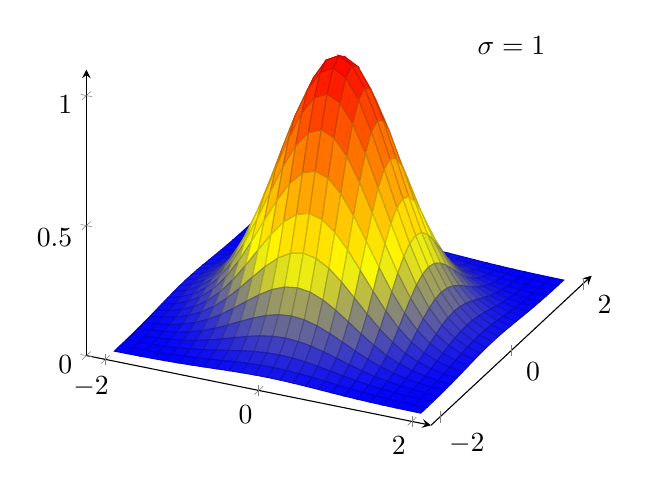
\begin{tikzpicture}

            \begin{axis}[
                    width=8cm,height=8cm,
                    domain=-2:2,
                    xmax=2.25,
                    ymax=2.25,
                    xmin=-2.25,
                    ymin=-2.25,
                    zmax=1.1,
                    axis lines = left,
                    colormap/hot,
                ]

                \addplot3[samples = 25, surf] {exp(-(x^2 + y^2)/1)};
                \node at (rel axis cs:1,0.5,1) [above] {\(\sigma=1\)};

            \end{axis}

        \end{tikzpicture}
    }%
    \quad
    \subfloat{
        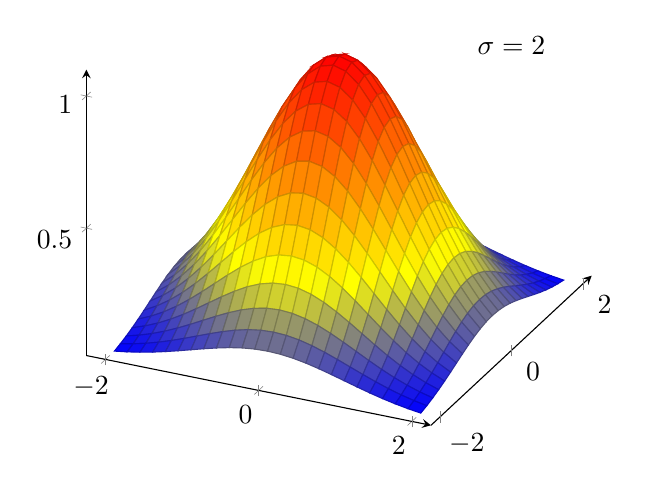
\begin{tikzpicture}

            \begin{axis}[
                    width=8cm,height=8cm,
                    domain=-2:2,
                    xmax=2.25,
                    ymax=2.25,
                    xmin=-2.25,
                    ymin=-2.25,
                    zmax=1.1,
                    axis lines = left,
                    colormap/hot,
                ]

                \addplot3[samples = 25, surf] {exp(-(x^2 + y^2)/2)};
                \node at (rel axis cs:1,0.5,1) [above] {\(\sigma=2\)};

            \end{axis}

        \end{tikzpicture}
    }%
    \caption{A graph of the Gaussian RBF from definition \ref{defe: grbfk} for $d=2$. Evidently, a larger value of $\sigma$ slows the rate of decay increasing the similarity between the same pair of samples.}%
    \label{fig: grbfk_graph_1}
\end{figure}

This kernel is infinitely differentiable meaning it has mean square derivatives of all orders and is therefore very smooth. In fact, some argue that such strong smoothness makes it unrealistic for modelling natural phenomena \cite{RasmussenCarlEdward2006Gpfm,SteinMichaelL1999IoSD}. Nontheless, Gaussian RBF kernelis still the one of the most widely used kernels in literature.

\subsection{Kernel Machines}\label{Section1.4}

In this section, we shall look at two different machine learning models that make use of kernels to perform classification and regression. The first kernel machine we shall look at are support vector machines (SVM). SVMs where originally designed for binary classification and as such we shall only present a model for binary classification, although extensions exist that allow regression and multi-class classification.

For the binary classification problem we are tasked with labelling new samples with either one of two classes, $-1$ or $1$. We shall assume our input space consists of vectors from $\RR^d$ and that we provided with a labelled training set $D = \left\{ \left( \bm{x}_1 , y_1 \right), \left( \bm{x}_1 , y_1 \right), \ldots , \left( \bm{x}_n , y_n \right) \right\}$. One simple method to classify samples is by creating an affine linear hyperplane satisfying
\begin{align} \label{eq: linear_sep_hyp}
    \langle \bm{w}, \bm{x}_i \rangle + b > 0, \quad y_i = +1 \nonumber \\
    \langle \bm{w}, \bm{x}_i \rangle + b < 0, \quad y_i = -1
\end{align}
for some $\bm{w} \in \RR^d$ and $b \in \RR$ where $\norm{w}_2 = 1$. Moreover we would like $\bm{w}$ and $b$ to maximise the margin, that is the maximal distance between the separating hyperplane and the points in $D$. The specific $\bm{w}$ and $b$ obtained through the training set is denoted $\bm{w}_D$ and $b_D$ and the resulting descision function is defined as
\[
    f_D \left( \bm{x} \right) \triangleq \operatorname{sign} \left( \langle \bm{w}_D , \bm{x} \rangle + b_D \right).
\]
There are, however, a number of short comings to this model. The most obvious is that our training data may not be linearly separable in $\RR^d$ meaning that no such $\bm{w}_D$ and $b_D$ exist. Moreover, when noise is introduced to the data set this model will prioritize finding a hyperplane that perfectly separates the two classes, making no comprises in misclassifying points, leaving it subject to overfitting. SVMs where introduced by Boser {\it et al.} \cite{BoserBernhard1992Ataf} to address the first issue of separability. Their approach was to lift the input vector into a more malleable Hilbert space $H_0$ using a feature map. The inputs are then classified within the new space. Unfortunately this method does nothing to address the second issue of over fitting and, if anything, actually worsens it. Cortes and Vapnik \cite{CortesCorinna1995SN} attempted to address this second issue by introducing slack variables to equation \ref{eq: linear_sep_hyp} so that we instead need to satisfy $y_i \left( \langle \bm{w} , \Phi \left( \bm{x}_i \right) \rangle + b \right) \geq 1 - \xi_i$ for some $\xi_i \in \RR_{>0}$. These constraints can be re-written as
\[
    \xi_i \geq 1 - y_i \left( \langle \bm{w} , \Phi \left( \bm{x}_i \right) \rangle + b \right)
\]
and combining this this our slack constraints (that is $\xi_i \geq 0$) yields
\[
    \xi_i \geq \max \left\{ 0, 1 - y_i \left( \langle \bm{w} , \Phi \left( \bm{x}_i \right) \rangle + b \right)  \right\} = L_{\text{hinge}} \left( y_i , \langle \bm{w} , \Phi \left( \bm{x}_i \right) \rangle + b \right)
\]
where $L_{\text{hinge}}$ is the hinge loss defined as
\[
    L_{\text{hinge}} \left( y,\eta \right) \triangleq \max \left\{ 0,1-y\eta \right\}.
\]
This optimization problem can be re-written is the form
\[
    \min_{\left( \bm{w} , b \right) \in H_0 \times \RR} \lambda \norm{\bm{w}}_{H_0} + \frac{1}{n} \sum_{i=1}^{n} L_{\text{hinge}} \left( y_i , f_{\left( \bm{w} , b \right)} \right)
\]
where $f_{\left( \bm{w} , b \right)} : X \to \RR$ is defined as
\[
    f_{\left( \bm{w} , b \right)} \triangleq \langle \bm{w} , \Phi \left( x_i \right) \rangle + b.
\]
Unfortunately, this new embedding requires us to solve for optimal parameters in a very high, or even infinite, dimension vector space. To get around this, often the Lagrange approach is used to solve the corresponding dual problem. When the hinge loss is used the dual problem becomes
\begin{align} \label{eq: SVM_dual_1}
     & \max_{\alpha \in \left[ 0,C \right]^n} \sum_{i=1}^{n} \alpha_i - \frac{1}{2} \sum_{i,j=1}^{n} y_i y_j \alpha_i \alpha_j \langle \Phi \left( \bm{x}_i \right), \Phi \left( \bm{x}_j \right) \rangle \nonumber \\
     & \text{subject to} \quad \sum_{i=1}^{n} y_i \alpha_i = 0
\end{align}
Notice that in the dual problem, we find that inner products are only taken with vectors that have the feature map applied to them allowing us to employ the kernel if the corresponding kernel trick described in section \ref{Section1.1} is known for the feature map used so that \ref{eq: SVM_dual_1} becomes
\begin{align*}
     & \max_{\alpha \in \left[ 0,C \right]^n} \sum_{i=1}^{n} \alpha_i - \frac{1}{2} \sum_{i,j=1}^{n} y_i y_j \alpha_i \alpha_j k \left( \bm{x}_i, \bm{x}_j \right) \\
     & \text{subject to} \quad \sum_{i=1}^{n} y_i \alpha_i = 0.
\end{align*}

The next machine learning model of interest that uses kernels are gaussian processes. To motivate this model, consider the time series data in figure \ref{fig: motive_gp_1}.

\begin{figure}[H]
    \centering
    \subfloat[]{
        \begin{tikzpicture}
            \draw[->,thick] (-0.01,0)--(6,0) node[right]{$x$};
            \draw[->,thick] (0,-0.01)--(0,6) node[above]{$y$};

            \draw[-,ultra thick] (0.7,-0.1)--(0.7,0.1) node[below,yshift=-0.3cm]{$x_1$};
            \draw[fill,draw,blue] (0.7,0.5) circle[radius=2.5pt];

            \draw[-,ultra thick] (1.4,-0.1)--(1.4,0.1) node[below,yshift=-0.3cm]{$x_2$};
            \draw[fill,draw,blue] (1.4,0.6) circle[radius=2.5pt];

            \draw[-,ultra thick] (2.7,-0.1)--(2.7,0.1) node[below,yshift=-0.3cm]{$x_3$};
            \draw[fill,draw,blue] (2.7,1.7) circle[radius=2.5pt];

            \draw[-,ultra thick] (3.7,-0.1)--(3.7,0.1) node[below,yshift=-0.2cm]{$x^{\ast}$};
            \draw[dashed,thick,red] (3.7,0)--(3.7,5);

            \draw[-,ultra thick] (5,-0.1)--(5,0.1) node[below,yshift=-0.3cm]{$x_4$};
            \draw[fill,draw,blue] (5,4) circle[radius=2.5pt];
        \end{tikzpicture}
    }%
    \qquad
    \subfloat[]{
        \begin{tikzpicture}
            \draw[->,thick] (-0.01,0)--(6,0) node[right]{$x$};
            \draw[->,thick] (0,-0.01)--(0,6) node[above]{$y$};

            \draw[-,ultra thick] (0.7,-0.1)--(0.7,0.1) node[below,yshift=-0.3cm]{$x_1$};
            \draw[fill,draw,blue] (0.7,0.5) circle[radius=2.5pt];
            \draw[dashed,blue] (0.7,0)--(0.7,4.7);
            \draw[<->,thick] (0.7,4.7)--(3.7,4.7) node[above,xshift=-1.5cm]{$k(x^{\ast},x_1)$};

            \draw[-,ultra thick] (1.4,-0.1)--(1.4,0.1) node[below,yshift=-0.3cm]{$x_2$};
            \draw[fill,draw,blue] (1.4,0.6) circle[radius=2.5pt];
            \draw[dashed,blue] (1.4,0)--(1.4,3.5);
            \draw[<->,thick] (1.4,3.5)--(3.7,3.5) node[above,xshift=-1.1cm]{$k(x^{\ast},x_2)$};

            \draw[-,ultra thick] (2.7,-0.1)--(2.7,0.1) node[below,yshift=-0.3cm]{$x_3$};
            \draw[fill,draw,blue] (2.7,1.7) circle[radius=2.5pt];
            \draw[dashed,blue] (2.7,0)--(2.7,2.3);
            \draw[<->,thick] (2.7,2.3)--(3.7,2.3) node[above,xshift=-0.9cm]{$k(x^{\ast},x_3)$};

            \draw[-,ultra thick] (3.7,-0.1)--(3.7,0.1) node[below,yshift=-0.2cm]{$x^{\ast}$};
            \node[diamond,draw,fill,draw,red,minimum width = 1cm,minimum height = 1.3cm,scale=0.25] (d) at (3.7,3) {};
            \draw[dashed,thick,red] (3.7,0)--(3.7,5);

            \draw[-,ultra thick] (5,-0.1 )--(5,0.1) node[below,yshift=-0.3cm]{$x_4$};
            \draw[fill,draw,blue] (5,4) circle[radius=2.5pt];
            \draw[dashed,blue] (5,0)--(5,4.5);
            \draw[<->,thick] (3.7,4.5)--(5,4.5) node[above,xshift=-0.3cm]{$k(x^{\ast},x_4)$};
        \end{tikzpicture}
    }%
    \caption{A graph of the Gaussian RBF from definition \ref{defe: grbfk} for $d=2$. Evidently, a larger value of $\sigma$ slows the rate of decay increasing the similarity between the same pair of samples.}%
    \label{fig: motive_gp_1}
\end{figure}

\begin{filecontents*}{./data/gp_intro_dat1.csv}
    x,y0,y1,y2
    0.0,3.8889447299776054,3.252195675396163,2.5723986201044187
    0.10204081632653061,3.8963153731866624,3.2334114175675395,2.4977761527857716
    0.20408163265306123,3.904676475191245,3.2263277175862597,2.4161726074738854
    0.30612244897959184,3.912486422260641,3.2265022294195966,2.3292200441690207
    0.40816326530612246,3.9181367775658873,3.228192583362307,2.2398507798591534
    0.5102040816326531,3.920256370846241,3.2249223304542913,2.152200525625582
    0.6122448979591837,3.9179701155023157,3.2101098230475538,2.071344891386562
    0.7142857142857143,3.9110778971645765,3.1777033459669783,2.0028774256062816
    0.8163265306122449,3.9001283490397016,3.122766415820061,1.9523672809629247
    0.9183673469387755,3.886376053031046,3.04196343041673,1.924753149634383
    1.0204081632653061,3.8716211994498333,2.933909038317024,1.9237443590136485
    1.1224489795918369,3.857954079608229,2.799351626306004,1.9513035606887854
    1.2244897959183674,3.847436905468257,2.6411768356723235,2.0072815139900495
    1.3265306122448979,3.841775787363871,2.4642319083119633,2.0892569830605368
    1.4285714285714286,3.8420321968485376,2.2749858593824617,2.192613833596985
    1.5306122448979593,3.8484268708760094,2.081057401633018,2.310856060666622
    1.6326530612244898,3.8602681088894766,1.8906546442626817,2.436135561712868
    1.7346938775510203,3.876016440194414,1.7119803587951616,2.559934911031695
    1.836734693877551,3.8934729250514666,1.5526570590488398,2.6738332705910244
    1.9387755102040818,3.9100510027824393,1.4192260798320049,2.7702684624537106
    2.0408163265306123,3.9230775813589482,1.3167595333633981,2.8432111425013322
    2.142857142857143,3.9300643637480857,1.248613256762677,2.888679554257369
    2.2448979591836737,3.9289011237509577,1.2163272198562576,2.905046033347129
    2.3469387755102042,3.9179401795449396,1.2196699093041794,2.8931101011392846
    2.4489795918367347,3.8959727008352174,1.2568027645405968,2.855945899531336
    2.5510204081632653,3.8621237371394623,1.3245411459916354,2.7985513820415195
    2.6530612244897958,3.8157151558884888,1.418678279406553,2.7273502460278247
    2.7551020408163267,3.756152285749804,1.5343452363886438,2.6496002463865618
    2.857142857142857,3.682888390340987,1.6663820121189532,2.5727700517645653
    2.9591836734693877,3.595495808498078,1.809697591321269,2.5039341546455005
    3.0612244897959187,3.493850568209357,1.9596010720146781,2.449232028447514
    3.163265306122449,3.378399275439287,2.1120883798539003,2.413420573364779
    3.2653061224489797,3.250456289718835,2.2640650594565668,2.3995428209525658
    3.36734693877551,3.1124629519607803,2.4134903440220477,2.4087275907808734
    3.4693877551020407,2.968139731618476,2.559424609970991,2.4401239977854456
    3.5714285714285716,2.8224826195273596,2.701970562220883,2.4909781807485927
    3.673469387755102,2.6815760504255355,2.8421022219924184,2.556846086350459
    3.7755102040816326,2.5522348648343,2.9813911671556212,2.6319349647504673
    3.8775510204081636,2.441513722741859,3.1216501445256846,2.709555194481732
    3.979591836734694,2.3561485591504203,3.264528290179406,2.7826529438164505
    4.081632653061225,2.3020051023456194,3.4111042700896737,2.8443841134520453
    4.183673469387755,2.2836063990304716,3.5615279847182504,2.8886791623908876
    4.285714285714286,2.3037932704691393,3.7147625310871684,2.9107453218748542
    4.387755102040816,2.3635503438936984,3.8684692167316403,2.907454656505577
    4.4897959183673475,2.461999004872191,4.019063544907245,2.8775731008424583
    4.591836734693878,2.596536742969357,4.161947681776214,2.821805978895311
    4.6938775510204085,2.763082806314141,4.291903941920607,2.742656025464969
    4.795918367346939,2.9563825813547977,4.4036048056748225,2.644116725967176
    4.8979591836734695,3.1703270754187236,4.492179720561176,2.5312380314160974
    5.0,3.398251248127017,4.553760976976619,2.4096316234579827
\end{filecontents*}

\begin{tikzpicture}
    \begin{axis}[
            xmin=-0.0,xmax=6.5,
            ymin=-0.5,ymax=6.5,
            axis line style={draw=none},
            tick style={draw=none},
            yticklabels=\empty,
            xticklabels=\empty,
        ]
        \addplot[smooth, color=black, semithick] table [x=x, y=y0, col sep=comma, mark=none] {./data/gp_intro_dat1.csv};
        \addplot[smooth, color=black, semithick, dashed] table [x=x, y=y1, col sep=comma, mark=none] {./data/gp_intro_dat1.csv};
        \addplot[smooth, color=black, semithick, dotted] table [x=x, y=y2, col sep=comma, mark=none] {./data/gp_intro_dat1.csv};
    \end{axis}
    \draw[->,thick] (0,0.5)--(0,5.5) node[above]{$y$};
    \draw[->,thick] (0,0.5)--(6,0.5) node[right]{$x$};
\end{tikzpicture}


\subsection{Gaussian Processes for Regression}\label{Section1.5}

We saw in section \ref{Section1.4} that, unlike most other machine learning models, GPs infer over a distribution of functions $p \left( f \mid D \right)$ instead of a vector of parameteric values $p \left( \bm{\theta} \mid D \right)$. Naively, one may attempt to find a suitable $f$ by fixing a class of functions $\calF$ and then search over this class to find a function that best represents the data. However, this may not work well if there is not enough richness in $\calF$ to represent the data. Instead we choose a suitable $f$ by assigning a prior probability to every possible function using the training data and then to select the function with the highest probability. To keep this computation tractable we only evalute our predicted function at a finite number of points. The prediction itself is found by taking the mean over all functions with respect to the posterior conditioned on the observed data which is assumed to be jointly Gaussian with the input value. This gives rise to Gaussian Process more formally stated in definition \ref{defe: GP}.

\begin{defe}[Gaussian Process] \label{defe: GP}
    A Gaussian Process (GP) is a collection of random variables with index set $I$, such that every finite subset of random variables has a joint Gaussian distribution \cite{RasmussenCarlEdward2006Gpfm,MurphyKevinP2012Ml}.
\end{defe}

A GP is completely characterised by a mean function $m(\bm{x})$ and a kernel, which in the context of GPs is sometimes called a covariance function, $k (\bm{x}, \bm{x'})$ on a real process as
\begin{align*}
    m(\bm{x})           & = \EE \left[ f(\bm{x}) \right]                                         \\
    k (\bm{x}, \bm{x'}) & = \EE \left[ (f(\bm{x}) - m(\bm{x})) (f(\bm{x'}) - m(\bm{x'})) \right]
\end{align*}
GPs define a prior over all possible functions which can be used to create a posterior once enough data has been observed. The prior is used to represent the functions we expect to see before any observations are made. Although defining a prior over all possible function may seem computationally intractable, we actually only need to define a distribution over a finite number of points. Before any observations are made, we typically assume that the mean function is the constant zero function, that is $m \left( \bm{x} \right) = 0$. A function $f(\bm{x})$ sampled from a GP with mean $m(\bm{x})$ and covariance $k (\bm{x}, \bm{x'})$ is written as
\[
    f(\bm{x}) \sim \calG \calP \left( m(\bm{x}), k (\bm{x}, \bm{x'}) \right)
\]
Since a GP is a collection of random variables it must satisfy the consistency requirement, that is, an observation of a set of variables should not the distribution of any small sub set of the observed values. More specifically if
\[
    (\bm{y_1}, \bm{y_2}) \sim \calN (\bm{\mu}, \bm{\Sigma})
\]
then
\begin{align*}
    \bm{y_1} & \sim \calN (\bm{\mu_1}, \bm{\Sigma_{1,1}}) \\
    \bm{y_2} & \sim \calN (\bm{\mu_2}, \bm{\Sigma_{2,2}})
\end{align*}

where $\bm{\Sigma_{1,1}}$ and $\bm{\Sigma_{2,2}}$ are the relevant sub matrices. Again, we shall us the notation that for set of data $\bm{W} = \left[ \bm{w}_1 ,\bm{w}_2 , \ldots , \bm{w}_n \right]^{\intercal} \in \RR^{n \times d}$ and $\bm{W}' = \left[ \bm{w}_1' ,\bm{w}_2' , \ldots , \bm{w}_m' \right]^{\intercal} \in \RR^{n' \times d}$ we use the notation
\[
    \left( \bm{K}_{\bm{W} \bm{W}'} \right)_{i,j} \triangleq k \left( \bm{w}_i , \bm{w}_j' \right)
\]
where \( \bm{K}_{\bm{W} \bm{W}'} \in \RR^{n \times n'} \). The convariance function completely characterized by its kernel. Unless otherwise stated, the kernel or covariance function used in examples and experimentation in the Gaussian RBF kernel, definition \ref{defe: grbfk}. To understand this better, as a small exercise we can select a number of inputs $\bm{X}^{\star} = \left[ \bm{x}_1 , \bm{x}_2 , \ldots , \bm{x}_{n^{\star}} \right]^{\intercal} \in \RR^{n^{\star} \times d}$ of compute the corresponding covariance matrix using the Gaussian RBF kernel. Gaussian vectors can then be sampled using a joint Gaussian distribution using the covariance matrix from the distribution
\[
    \bm{f}^{\star} \sim \calN \left( \bm{0}, \bm{K_{X^{\star} X^{\star}}} \right)
\]
graph its values as a function of its inputs.

\begin{filecontents*}{./data/gp_intro_dat1.csv}
    x,y0,y1,y2
    0.0,2.6341780930873786,4.41685044685407,1.884123117075101
    0.11224489795918367,2.685150340856032,4.351109330694541,2.0933788453347146
    0.22448979591836735,2.758222906849677,4.246986054733594,2.3215583495507697
    0.336734693877551,2.844091796198551,4.111722477611423,2.5621308980348045
    0.4489795918367347,2.9327004798948444,3.954138391914307,2.8093607381581323
    0.5612244897959183,3.0142490315111,3.7837568463624893,3.058296829896802
    0.673469387755102,3.0800293333419133,3.609905398833131,3.304575221937234
    0.7857142857142857,3.1230071846450134,3.4408573216000065,3.5440886761610075
    0.8979591836734694,3.1381275068842287,3.2830844115325393,3.772606115615495
    1.010204081632653,3.1223796951701805,3.1407028040204787,3.985434762859824
    1.1224489795918366,3.074690487867501,3.0151840031490704,4.177213384641246
    1.2346938775510203,2.99572649694323,2.9053883056890326,4.341906534238328
    1.346938775510204,2.887680093346262,2.807934404050683,4.473021654529128
    1.4591836734693877,2.7540712359611135,2.7178753181761683,4.5640359352552755
    1.5714285714285714,2.5995639802641644,2.629596908378246,4.608968085491204
    1.683673469387755,2.4297636797240854,2.537815790076743,4.603008456947798
    1.7959183673469388,2.250945266539242,2.4385306514757277,4.54310273176884
    1.9081632653061225,2.0696826217289814,2.3297825969976156,4.428402138611055
    2.020408163265306,1.8923794707563157,2.2121155584786374,4.26051300065903
    2.13265306122449,1.724750314129252,2.088670901030661,4.043522033936433
    2.2448979591836733,1.5713409480295042,1.9649185604698398,3.78380984825793
    2.357142857142857,1.4351902937232137,1.8480772970914263,3.4896953544368947
    2.4693877551020407,1.3177316537250037,1.7463209648090843,3.170973707657322
    2.5816326530612246,1.2189781885886188,1.667887909534986,2.838411584600058
    2.693877551020408,1.137982180009872,1.6202034591848866,2.503253609595508
    2.806122448979592,1.0734814750833834,1.6091067041507867,2.176777775544475
    2.9183673469387754,1.0246008560812094,1.638242628202587,1.8699164299237567
    3.0306122448979593,0.9914469543413351,1.708653796550625,1.5929463528940093
    3.142857142857143,0.9754532832118712,1.8185871450769515,1.3552308689036683
    3.2551020408163267,0.9793831046385866,1.9635250522558478,1.1649988273056024
    3.36734693877551,1.0069633897912214,2.136445411268843,1.0291341361289352
    3.479591836734694,1.0622134340832736,2.328310102622806,0.9529576266820667
    3.5918367346938775,1.1485904962060034,2.5287676666005745,0.9399816624503701
    3.704081632653061,1.2681182060719118,2.7270230125223396,0.9916380696381344
    3.816326530612245,1.4206777569266578,2.9127943188682153,1.1069890129419622
    3.9285714285714284,1.603600797665261,3.077239529790242,1.282461239660869
    4.040816326530612,1.8116633596458505,3.213718985997705,1.5116563075035667
    4.153061224489796,2.0374945244629954,3.31826875093589,1.7853109321561014
    4.26530612244898,2.272346385818944,3.3896996920659737,2.0914743830547122
    4.377551020408164,2.50710273056381,3.4293088690936613,2.415953795652976
    4.489795918367347,2.7333622652331386,3.440263336916595,2.743037053839629
    4.6020408163265305,2.9444150750492786,3.426788503862636,3.0564529194286605
    4.714285714285714,3.1359501955059153,3.3933321658244284,3.3404756976868217
    4.826530612244898,3.306372509617609,3.343882098004392,3.5810500536442835
    4.938775510204081,3.456677113806286,3.281564998201946,3.766794718394943
    5.051020408163265,3.5899014357864862,3.2085942528948497,3.889767236618262
    5.163265306122449,3.710253447229357,3.1265441378249808,3.9459164775264113
    5.275510204081633,3.822067924064683,3.036856306931041,3.9352029543435254
    5.387755102040816,3.928774395166681,2.9414323013414645,3.8614290770863415
    5.5,4.032057566247807,2.843156622782664,3.7318467351526268
\end{filecontents*}

\begin{filecontents*}{./data/gp_intro_dat2.csv}
    x,mu,y0,y1,y2,bU,bL
    0.0,2.96787109791578,3.646442446207024,2.3796779884645356,3.123887098083909,3.8222957144465917,2.1134464813849685
    0.11224489795918367,3.178846435851742,3.7278533056947927,2.705139783400845,3.3197136652913843,3.8425540443223007,2.515138827381183
    0.22448979591836735,3.373957062754166,3.772122911137243,3.033674383762561,3.4864096188544065,3.8416203985733905,2.906293726934942
    0.336734693877551,3.550670833185919,3.7845706480846375,3.3482893361633472,3.6227538754415383,3.8226477418327116,3.2786939245391267
    0.4489795918367347,3.707387470227142,3.777024821961083,3.6497714076425667,3.734021204276469,3.7908281722625117,3.623946768191772
    0.5612244897959183,3.8435001880813098,3.7587623765632605,3.9224326540622303,3.820415281746996,3.938789896922746,3.7482104792398734
    0.673469387755102,3.959374699757277,3.7401691473547714,4.161761533893699,3.884187912930478,4.2112638754378935,3.70748552407666
    0.7857142857142857,4.056245238332488,3.727886967246087,4.3591514373501585,3.9294944134700884,4.440290931214802,3.6721995454501735
    0.8979591836734694,4.136035742591053,3.7320230213633776,4.516870894977162,3.9667169440013335,4.6225623417878845,3.6495091433942224
    1.010204081632653,4.201122318895088,3.7511336294964686,4.631536079365145,3.9909291094494637,4.756943867968448,3.645300769821728
    1.1224489795918366,4.254059537569402,3.7922886212348805,4.703821106353732,4.014456904551665,4.844164391874928,3.663954683263876
    1.2346938775510203,4.297297268072625,3.8510310641448773,4.736836098027459,4.040882180292408,4.886718646421257,3.7078758897239927
    1.346938775510204,4.332916090251523,3.931146658869461,4.737917134427073,4.0721402987298845,4.8886932140093196,3.7771389664937254
    1.4591836734693877,4.362407665942143,4.019692223676497,4.711145152040588,4.114354849026403,4.855508162034269,3.869307169850018
    1.5714285714285714,4.386522000140943,4.113994631302509,4.667147410140193,4.1675113923767135,4.79358919579317,3.9794548044887157
    1.683673469387755,4.405196773426522,4.211161115648332,4.60858632272203,4.2301483229724735,4.709995085814498,4.100398461038546
    1.7959183673469388,4.417575648333239,4.297237502243545,4.542647493156313,4.298601004588312,4.612045273426419,4.223106023240059
    1.9081632653061225,4.422113551855313,4.370044631852721,4.478504417000914,4.366233750854552,4.507185391473455,4.337041712237171
    2.020408163265306,4.416758358107319,4.4212535412567835,4.413073469318789,4.428720525173312,4.439002309014812,4.394514407199825
    2.13265306122449,4.399191007367498,4.4498214644109035,4.354633815643454,4.472837424274621,4.501454599238494,4.296927415496501
    2.2448979591836733,4.367100601462363,4.44669502086167,4.293220973455457,4.495071115055989,4.529355328572067,4.204845874352659
    2.357142857142857,4.318467882753287,4.4122754488830465,4.2367626348642995,4.480392701402552,4.511998980020114,4.124936785486461
    2.4693877551020407,4.251829947856004,4.344361140161457,4.176480274188317,4.420872228223025,4.444440701959786,4.059219193752223
    2.5816326530612246,4.166501022807468,4.242712341391929,4.110274997773214,4.315673648503417,4.324777879750019,4.008224165864918
    2.693877551020408,4.062728357957119,4.110217875771083,4.032563200602017,4.153918593320322,4.154406402240164,3.9710503136740742
    2.806122448979592,3.9417683270387145,3.9492135726749384,3.9344120355000705,3.9443400697750968,3.9571937560826638,3.926342897994765
    2.9183673469387754,3.805875044263767,3.7642279401126544,3.810832282328448,3.684817080524404,3.9345310053498097,3.6772190831777247
    3.0306122448979593,3.6582015833339296,3.564842924761986,3.6644624038944493,3.3833530964865193,3.9269741902831705,3.3894289763846888
    3.142857142857143,3.5026215163692607,3.3520647108430026,3.488370188345563,3.052946676019309,3.9234237680191817,3.0818192647193396
    3.2551020408163267,3.3434853499709174,3.1402141378498163,3.2837887833202726,2.7002390009588226,3.920293063216916,2.7666776367249186
    3.36734693877551,3.1853319635639767,2.934150639260623,3.057322775625835,2.3472996257286054,3.914233966397971,2.4564299607299827
    3.479591836734694,3.03257891484487,2.738827249921258,2.812094834179371,2.009196676123942,3.902114762761585,2.163043066928155
    3.5918367346938775,2.8892171796754873,2.5662919443248073,2.559707152254641,1.6967015390942675,3.881056263819646,1.8973780955313282
    3.704081632653061,2.758535417727554,2.41434042449297,2.309411800258502,1.4256334316849872,3.848437973565799,1.668632861889309
    3.816326530612245,2.642896256015177,2.2902148380401837,2.075552115650442,1.207890471342624,3.8018786148254615,1.4839138972048924
    3.9285714285714284,2.5435825902305362,2.1965744091641124,1.8662299680038845,1.0467598332277432,3.7392081008329594,1.3479570796281128
    4.040816326530612,2.4607259083694415,2.133954232173078,1.6922651032951084,0.952486845042865,3.6584498086819774,1.2630020080569058
    4.153061224489796,2.393321664023437,2.0881938587934696,1.566133253333461,0.92147130773977,3.5578289289014684,1.2288143991454055
    4.26530612244898,2.339329380270647,2.0632588371219063,1.4903968555363714,0.94987473663854,3.435816329632721,1.2428424309085735
    4.377551020408164,2.295848100924048,2.0605594124527933,1.4690236774181895,1.033187881225276,3.2912091804701387,1.3004870213779576
    4.489795918367347,2.259351656203322,2.064341290936802,1.499164363108256,1.1636813952423448,3.123241143061824,1.3954621693448201
    4.6020408163265305,2.2259635269573055,2.0739080755801877,1.575649936757477,1.3294049093439706,2.931708042701583,1.520219011213028
    4.714285714285714,2.1917482915683912,2.0845379827266677,1.6904928495001776,1.5224847717101069,2.717092081155121,1.6664045019816616
    4.826530612244898,2.1529959577040843,2.0900622587437008,1.8320811599608942,1.733755447747318,2.4806793091811996,1.8253126062269691
    4.938775510204081,2.10647694342231,2.087733094036374,1.98722071801456,1.9517354055585423,2.2248945171189956,1.988059369725624
    5.051020408163265,2.049648890548753,2.0747166503580527,2.1438285289379833,2.167467964578078,2.149507699667685,1.9497900814298208
    5.163265306122449,1.9808014834652514,2.050810263655156,2.283421101970534,2.3742039664111614,2.297682746932975,1.663920219997528
    5.275510204081633,1.8991314699538484,2.006424555553889,2.395089681917207,2.5656201066053885,2.429871221330997,1.3683917185766998
    5.387755102040816,1.8047465055032903,1.9408588788404912,2.4682291512970815,2.7418915989000654,2.5411728761483077,1.068320134858273
    5.5,1.69860261545027,1.8531818596862015,2.488627885130089,2.8888780190386125,2.628636682030301,0.7685685488702394
\end{filecontents*}

\begin{figure}[h]
    \centering
    \subfloat[]{
        \begin{adjustbox}{width=0.48\textwidth}
            \begin{tikzpicture}[>=latex]
                \begin{axis}[
                        xmin=-0.0,xmax=6.5,
                        ymin=-0.5,ymax=6.5,
                        axis line style={draw=none},
                        tick style={draw=none},
                        yticklabels=\empty,
                        xticklabels=\empty,
                    ]
                    \addplot[smooth, color=black, semithick] table [x=x, y=y0, col sep=comma, mark=none] {./data/gp_intro_dat1.csv};
                    \addplot[smooth, color=black, semithick, dashed] table [x=x, y=y1, col sep=comma, mark=none] {./data/gp_intro_dat1.csv};
                    \addplot[smooth, color=black, semithick, dotted] table [x=x, y=y2, col sep=comma, mark=none] {./data/gp_intro_dat1.csv};

                    \addplot[name path = bU, mark=none, blue!10] coordinates {(0,0.5) (5.5,0.5)};
                    \addplot[name path = bL, mark=none, blue!10] coordinates {(0,5.75) (5.5,5.75)};
                    \addplot [blue!10] fill between [of = bU and bL, soft clip={domain=0:5.5}];

                \end{axis}
                \draw[color=red, ultra thick] (0,3)--(5.8,3);
                \draw[->,thick] (0,0.5)--(0,5.5) node[above]{$y$};
                \draw[->,thick] (0,0.5)--(6,0.5) node[right]{$x$};
            \end{tikzpicture}
        \end{adjustbox}
    }
    \subfloat[]{
        \begin{adjustbox}{width=0.48\textwidth}
            \begin{tikzpicture}[>=latex]
                \begin{axis}[
                        xmin=-0.0,xmax=6.5,
                        ymin=-0.5,ymax=6.5,
                        axis line style={draw=none},
                        tick style={draw=none},
                        yticklabels=\empty,
                        xticklabels=\empty,
                    ]
                    \addplot[smooth, color=black, semithick] table [x=x, y=y0, col sep=comma, mark=none] {./data/gp_intro_dat2.csv};
                    \addplot[smooth, color=black, semithick, dashed] table [x=x, y=y1, col sep=comma, mark=none] {./data/gp_intro_dat2.csv};
                    \addplot[smooth, color=black, semithick, dotted] table [x=x, y=y2, col sep=comma, mark=none] {./data/gp_intro_dat2.csv};
                    \addplot[smooth, color=red, ultra thick] table [x=x, y=mu, col sep=comma, mark=none] {./data/gp_intro_dat2.csv};

                    \addplot[name path = bU, smooth, color=blue!10] table [x=x, y=bU, col sep=comma, mark=none] {./data/gp_intro_dat2.csv};
                    \addplot[name path = bL, smooth, color=blue!10] table [x=x, y=bL, col sep=comma, mark=none] {./data/gp_intro_dat2.csv};
                    \addplot [blue!10] fill between [of = bU and bL, soft clip={domain=0:5.5}];
                \end{axis}
                \draw[->,thick] (0,0.5)--(0,5.5) node[above]{$y$};
                \draw[->,thick] (0,0.5)--(6,0.5) node[right]{$x$};
                \draw[-,ultra thick] (0.5,0.4)--(0.5,0.6) node[below,yshift=-0.3cm]{$x_1$};
                \draw[-,ultra thick] (2.1,0.4)--(2.1,0.6) node[below,yshift=-0.3cm]{$x_2$};
                \draw[-,ultra thick] (2.95,0.4)--(2.95,0.6) node[below,yshift=-0.3cm]{$x_3$};
                \draw[-,ultra thick] (5.3,0.4)--(5.3,0.6) node[below,yshift=-0.3cm]{$x_4$};

                \foreach \Point in {(0.5, 3.45), (2.1, 4.0), (2.95, 3.6), (5.3, 2.1)}{
                        \node at \Point {\contour{white}{\Large \textbf{+}}};
                    }
            \end{tikzpicture}
        \end{adjustbox}
    }
    \caption{Panel (A) shows three function drawn from the prior distribution. Panel (B) shows three function drawn from the prior distribution after four observations have been made. In both panels the mean function is drawn in red, sampled functions in black and twice the standard deviation shaded in light blue.}
    \label{fig: GP_func_samples}
\end{figure}

Figure \ref{fig: GP_func_samples} (A) shows three samples drawn from the prior before any observations are made. GPs also allow us to compute the pointwise variance which can provide some measure of variability for predicted values. The blue shaded area of figure \ref{fig: GP_func_samples} (A) represents twice the standard deviation about the mean.

\subsubsection{Noise-free observations}\label{Section1.5.1}
Typically when using GP we would like to incorporate data from observations, or training data, into our predictions on unobserved values.
Let us suppose there is some obsevered data $D = \left\{ (\bm{x}_i, \bm{f}_i) \mid i \in \left\{ 1,2, \ldots , n \right\} \right\}$ which is (unrealistically) noise-free that we would like to model as a GP. In other words, for any sample in our dataset we can be certain that the observed value is the true value of the underlying function we wish to model. Then for the observed data
\[
    \bm{f} \sim \calN \left( \bm{0}, \bm{K_{XX}} \right).
\]
We would then like to make a prediction for unobserved values say $X^{\star} = \left[ \bm{x}_1^{\star}, \bm{x}_2^{\star}, \ldots , \bm{x}_{n_\star}^{\star} \right]$ with value $f_{\star}$ as has a distribution of
\[
    \bm{f}_{\star} \sim \calN \left( \bm{0}, \bm{K_{X^{\star}X^{\star}}} \right).
\]
where $\bm{K_{X^{\star}X^{\star}}} = k(\bm{X^{\star}}, \bm{X^{\star}}) \in \RR^{n_\star \times n_\star}$. Here $\bm{f}$ and $\bm{f}_{\star}$ are independent but we would like to give them some sort of correlation. We can do this by having them originate from the same joint distribution. According to the prior, we can write the joint distribution of the training points $\bm{f}$ and the test points $\bm{f}_{\star}$ as
\[
    \begin{bmatrix}
        \bm{f} \\
        \bm{f}_{\star}
    \end{bmatrix}
    \sim \calN
    \begin{pmatrix}
        \bm{0}, &
        {
                \begin{bmatrix}
                    \bm{K_{XX}}                     & \bm{K_{XX^{\star}}}         \\
                    \bm{K_{XX^{\star}}}^{\intercal} & \bm{K_{X^{\star}X^{\star}}}
                \end{bmatrix}
            }
    \end{pmatrix}
\]
where $\bm{K_{XX^{\star}}} = k(\bm{X}, \bm{X^{\star}}) \in \RR^{n \times n_\star}$.

While the above does give us some information on $\bm{f}_{\star}$ is related to the observed data and the test inputs, it does not provide any method to evalute $\bm{f}_{\star}$. To do this we shall need the assistance of the following lemma
\begin{thm}\label{theorem: cond_of_MVN}
    (Marginals and conditionals of an MVN \cite{MurphyKevinP2012Ml}) Suppose $\bm{x} = (\bm{x}_1, \bm{x}_2)$ is jointly Gaussian with parameters
    \[
        \bm{\mu} =
        \begin{bmatrix}
            \bm{\mu}_1 \\
            \bm{\mu}_2
        \end{bmatrix}, \quad
        \bm{\Sigma} =
        \begin{bmatrix}
            \bm{\Sigma}_{1,1} & \bm{\Sigma}_{1,2} \\
            \bm{\Sigma}_{2,1} & \bm{\Sigma}_{2,2}
        \end{bmatrix}
    \]
    then the posterior conditional is given by
    \begin{align*}
        \bm{x}_2 \mid \bm{x}_1 & \sim \calN \left( \bm{x}_2 \mid \bm{\mu}_{2 \mid 1}, \bm{\Sigma}_{2 \mid 1} \right)          \\
        \bm{\mu}_{2 \mid 1}    & = \bm{\mu}_2 + \bm{\Sigma}_{2,1} \bm{\Sigma}_{1,1}^{-1} \left( \bm{x}_1 - \bm{\mu}_1 \right) \\
        \bm{\Sigma}_{2 \mid 1} & = \bm{\Sigma}_{2,2} - \bm{\Sigma}_{2,1} \bm{\Sigma}_{1,1}^{-1} \bm{\Sigma}_{1,2}
    \end{align*}
\end{thm}

Thus finding a mean an covariance for $\bm{f}_{\star}$ requires a direct application of Theorem \ref{theorem: cond_of_MVN} which gives
\begin{align*}
    \bm{f}_{\star} \mid \bm{K_{XX^{\star}}} , \bm{K_{XX}}, \bm{f} \sim \calN \left( \bm{\mu}^{\star}, \bm{\Sigma}^{\star} \right)
\end{align*}
where
\begin{align*}
    \bm{\mu}^{\star} & = \bm{0} + \bm{K_{XX^{\star}}}^{\intercal} \bm{K_{XX}}^{-1} \left( \bm{f} - \bm{0} \right) \\
                     & = \bm{K_{XX^{\star}}}^{\intercal} \bm{K_{XX}}^{-1} \bm{f}
\end{align*}
and
\begin{align*}
    \bm{\Sigma}^{\star} & = \bm{K_{X^{\star}X^{\star}}} - \bm{K_{XX^{\star}}}^{\intercal} \bm{K_{XX}}^{-1} \bm{K_{XX^{\star}}}
\end{align*}
meaning we can write a distribution for $\bm{f}_{\star}$ as
\begin{equation}\label{prop:GP_train_distr1}
    \bm{f}_{\star} \mid \bm{K_{XX^{\star}}} , \bm{K_{XX}}, \bm{f} \sim \calN \left( \bm{K_{XX^{\star}}}^{\intercal} \bm{K_{XX}}^{-1} \bm{f},  \bm{K_{X^{\star}X^{\star}}} - \bm{K_{XX^{\star}}}^{\intercal} \bm{K_{XX}}^{-1} \bm{K_{XX^{\star}}}  \right)
\end{equation}
Function values from the unobserved inputs $\bm{X^{\star}}$, that is $\bm{f}_{\star}$, can be estimated using the joint posterior distribution by evaulting the mean of \ref{prop:GP_train_distr1}. Figure \ref{fig: GP_func_samples} (B) shows these computations given a data set $D = \left\{ \left( x_1 , y_1 \right) , \left( x_2 , y_2 \right) , \left( x_3 , y_3 \right) , \left( x_4 , y_4 \right) \right\}$. Notice that the variance tightens around the observed values since (assuming no noise in our data is present) we know for certain this is how our target function should behave at $x_1,x_2,x_3$ and $x_4$. Specifying the properties of the prior is important since it fixes the properties of the functions considered during inference.

\subsubsection{Prediction with Noisy observations}\label{Section1.5.2}
When attempting to model our value function we usually do not have access to the value function itself but a noisy version thereof, $y = f(\bm{x}) + \varepsilon$ where $\varepsilon \sim \calN (0, \sigma_n^2)$ meaning the prior on the noisy values becomes
\[
    \operatorname{cov} (\bm{y}) = \bm{K_{XX}} + \sigma_n^2 \bm{I}
\]
The reason why noise is only added along the diagonal follows from the assumption of independence in our data.
We can write out the new distribution of the observed noisy values along the points at which we wish to test the underlying function as
\[
    \begin{bmatrix}
        \bm{y} \\
        \bm{f}_{\star}
    \end{bmatrix}
    \sim \calN
    \begin{pmatrix}
        \bm{0}, &
        {
                \begin{bmatrix}
                    \bm{K_{XX}} + \sigma_n^2 \Id_{n \times n} & \bm{K_{XX^{\star}}}         \\
                    \bm{K_{XX^{\star}}}^{\intercal}           & \bm{K_{X^{\star}X^{\star}}}
                \end{bmatrix}
            }
    \end{pmatrix}
\]
Using a similar we arrive at a similar condition distribution of $\bm{f}_{\star} \mid \bm{K_{XX^{\star}}} , \bm{K_{XX}}, \bm{f}$ we arrive at one of the most fundamental equations for GP regression tasks
\begin{equation}\label{prop:GP_train_distr2}
    \bm{f}_{\star} \mid \bm{K_{XX^{\star}}} , \bm{K_{XX}}, \bm{y} \sim \calN \left( \overline{\bm{f}_{\star}}, \operatorname{cov} (\bm{f}_{\star}) \right)
\end{equation}
where
\begin{align}
    \overline{\bm{f}_{\star}}           & \triangleq \bm{K_{XX^{\star}}}^{\intercal} \left[ \bm{K_{XX}} + \sigma_n^2 \Id_{n \times n} \right]^{-1} \bm{y} \label{eq: GP_train_distr2_mean}                                  \\
    \operatorname{cov} (\bm{f}_{\star}) & = \bm{K_{X^{\star}X^{\star}}} - \bm{K_{XX^{\star}}}^{\intercal} \left[ \bm{K_{XX}} + \sigma_n^2 \Id_{n \times n} \right]^{-1} \bm{K_{XX^{\star}}} \label{eq: GP_train_distr2_var}
\end{align}
Remarkably, this gives us the the exact same posterior distribution ascertained from the weight space derivation in equation \ref{eq: comput_f_ast_3}. Notice that the prediction of the mean in equation \ref{eq: GP_train_distr2_mean} is a linear combination of the observations, somtimes referred to as a {\it linear predictor}. Another way of looking at the prediction is seeing it as a linear combination of $n$ kernel evaluations centered at the input $\bm{x}^{\star}$
\[
    \bm{f}_{\star} = \sum_{i=1}^{n} \alpha_i k \left( \bm{x}_i , \bm{x}^{\ast} \right)
\]
where $\bm{\alpha} = \left[ \bm{K_{XX}} + \sigma_n^2 \Id_{n \times n} \right]^{-1} \bm{y}$. Intuitively, this expression can be understood by realising that despite defining the GP defining a joint Gaussian distribution over the observations when making predictions GPs only require the $(n+1)$-dimension distribution defined by the $n$ observations and the single test point. Marginalising by taking  the relevant submatrix block of the covariance matrix yields our desired $1$-dimensional prediction.

Also notice that the covariance does not depend on observations but scales quadratically to the norm of the testing inputs. This is a key feature of GPs. The variance is comprised of the difference between the prior covariance, $\bm{K_{X^{\star}X^{\star}}}$, and positive term $\bm{K_{XX^{\star}}}^{\intercal} \left[ \bm{K_{XX}} + \sigma_n^2 \Id_{n \times n} \right]^{-1} \bm{K_{XX^{\star}}}$ which represents knowledge given by the observations about the underlying function.

Algorithm \ref{alg: Unoptimized_GPR} shows one possible implementation for computing the mean and covariance of a single test input.

    {\centering
        \begin{minipage}{.85\linewidth}
            \begin{algorithm}[H]
                \caption{Unoptimized GPR}
                \label{alg: Unoptimized_GPR}
                \SetAlgoLined
                \DontPrintSemicolon
                \SetKwInOut{Input}{input}\SetKwInOut{Output}{output}

                \Input{Observations $\bm{X}, \bm{y}$ and a test input $\bm{x}^{\star}$.}
                \Output{A prediction $\overline{f_{\star}} $ with its corresponding variance $ \VV \left[ f_{\star} \right]$.}
                \BlankLine
                $\bm{L} = \operatorname{cholesky} \left( \bm{K_{XX}} + \sigma_n^2 \Id_{n \times n} \right)$\;
                $\bm{\alpha} = \operatorname{lin-solve} \left( \bm{L}^{\intercal} , \operatorname{lin-solve} \left( \bm{L}, \bm{y} \right) \right)$\;
                $\overline{f_{\star}} = \bm{K_{x^{\star} X}} \bm{\alpha}$\;
                $\bm{v} = \operatorname{lin-solve} \left( \bm{L}, \bm{K_{x^{\star} X}} \right)$\;
                $\VV \left[ f_{\star} \right] = \bm{K_{x^{\star} x^{\star}}} - \bm{v}^{\intercal} \bm{v}$\;
                \Return{$\overline{f_{\star}} , \VV \left[ f_{\star} \right]$}
                \BlankLine
            \end{algorithm}
        \end{minipage}
        \par
    }

A cholesky decomposition is typically used since $\bm{L}$ can be used twice to assist in solving both the linear systems in the mean and covariance. Unfortunately, a cholesky decomposition incurres a runtime of $\calO \left( n^3 \right)$ where $n$ is the number of samples making it impractical for large data sets. In the later chapters we shall consider other methods for solving these linear systems.

\subsection{Gaussian Processes for Classification}\label{Section1.6}

As with most classification models, the Gaussian processes classifier (GPC) seeks an estimate for the joint probability $p \left( y , \bm{x} \right)$ where $\bm{x} \in \RR^d$ is an input, as in the regression case, but $y$ is now a class taking on a discrete and finite number of values $\left\{ \calC_i \right\}_{i=1}^C$. Using Baye's theorem the joint probability density can be decomposed into either $p \left( y \right) p \left( \bm{x} \mid y \right)$ or $p \left( \bm{x} \right) p \left( \bm{y} \mid \bm{x} \right)$ giving rise to the {\it generative} and {\it discriminative} approaches respectively \cite{RasmussenCarlEdward2006Gpfm}*{page 34}. The generative approach models the prior probabilities of each class, $p \left( \calC_i \right)$, as well as the class conditional probabilities for each input $p \left( \bm{x} \mid \calC_i \right)$ and computes the posterior as
\[
    p \left( y \mid \bm{x} \right) = \frac{ p \left( y \right) p \left( \bm{x} \mid y \right) }{ \sum_{i=1}^{C} p \left( \calC_i \right) p \left( \bm{x} \mid \calC_i \right) }.
\]
On the other hand, the discriminative method focuses on modelling $p \left( y \mid \bm{x} \right)$ directly. With both these paradigms at our disposal, which one would be preferred for our GPC? While there are strengths and weaknesses associated with both models, the discriminative approach is usually chosen as it has a rather attractive property of directly modeling what we require, that is $p \left( y \mid \bm{x} \right)$. Aditionally, the density estimation of $p \left( \bm{x} \mid \calC_i \right)$ using in the generative model presents a number of difficulties, especially for larger values of $d$. If we are only focused on classifying inputs, the generative approach could mean trying to solve a harder problem than what is necessary. For this reason we focus on GPCs that adopt the discriminative approach.

\subsubsection{Linear Models for Classification}\label{Section1.6.1}

We can start by reviewing linear models for the simplist form of classification, that is binary classification. Adopting the notation from SVM (see section \ref{Section1.4.1}) literature, the binary classification problem involves assigning an input $\bm{x}$ to a class of either $-1$ or $+1$. For a linear model likelihood can be formulated as
\begin{equation} \label{eq: GPC-lin-model-1}
    p \left( y=+1 \mid \bm{x} , \bm{w} \right) = \sigma \left( \langle \bm{x} , \bm{w} \rangle \right)
\end{equation}
given a weight vector $\bm{w}$ and where $\sigma (\bm{z})$ is chosen to be any sigmoid function, see definition \ref{defe: sigmoid-function}.
\begin{defe}[Sigmoid Function] \label{defe: sigmoid-function}
    A sigmoid function is a monotonically increasing function mapping from $\RR$ to $\left[ 0,1 \right]$ \cite{RasmussenCarlEdward2006Gpfm}*{page 35}.
\end{defe}
In this text, the commonly used logistic function
\begin{equation} \label{eq: logistic-function}
    \sigma (z) = \frac{1}{1 + \exp (-z)}
\end{equation}
will take the role of the sigmoid function in equation \ref{eq: GPC-lin-model-1}, graphed in Figure \ref{fig: logistic-func-and-probit}. This type of model is aptly named the logistic regression.
\begin{figure}[h]
    \centering
    \begin{tikzpicture}[>=latex, scale=1.1]
        \begin{axis}[
                axis line style = thick,
                xlabel={$x$},
                ylabel={$y$},
                every axis x label/.style={
                        at={(ticklabel* cs:1.01)},
                        anchor=west,
                    },
                xmin=-5.5,xmax=5.5,
                ymin=-0.125,ymax=1.125,
                axis y line =middle,
                axis x line =bottom,
                every axis y label/.style={
                        at={(ticklabel* cs:1.01)},
                        anchor=south,
                    },
                % axis line style={->},
                xticklabels={$-5$, $5$},
                xtick={-5,5},
                yticklabels={$0$, $1$},
                ytick={-0.05,0.95},
                % axis line style={draw=none},
                ytick style={draw=none},
            ]
            \addplot[smooth, color=red, thick] {1/(1+exp(-x))};
            \addplot [smooth, blue, thick, dashed] {normcdf((0.6266 * x),0,1)};
            \addplot[smooth, color=black, semithick, dotted] {0};
            \addplot[smooth, color=black, semithick, dotted] {1};
        \end{axis}
    \end{tikzpicture}
    \caption{The logistic function from equation \ref{eq: logistic-function} (solid red) juxtaposed with a close approximation, the scaled probit function (dashed blue).}
    \label{fig: logistic-func-and-probit}
\end{figure}
Unlike GPR, the likelihood is no longer a Gaussian distribution. Instead it follows the Bernoulli distribution
\begin{equation*}
    p \left( y \mid \bm{x} , \bm{w} \right) = \sigma \left( \langle \bm{x} , \bm{w} \rangle \right)^{y} \left( 1 - \sigma \left( \langle \bm{x} , \bm{w} \rangle \right) \right)^{\frac{1 - y}{2}}
\end{equation*}
which for symmeteric likelihood functions can be written more concisely as
\begin{equation*}
    p \left( y_i \mid \bm{x}_i , \bm{w} \right) = \sigma \left( y_i f_i \right)
\end{equation*}
where
\begin{equation} \label{eq: GPC-lin-latent-func}
    f_i \triangleq f \left( \bm{x}_i \right) = \langle \bm{x} , \bm{w} \rangle .
\end{equation}
Thus, the logistic regression model can be written as the log ratio of the likelihoods of the input belonging to either class, that is
\begin{equation*}
    \operatorname{logit} \left( \bm{x} \right) \triangleq \langle \bm{x} , \bm{w} \rangle = \log \left( \frac{p \left( y = +1 \right)}{p \left( y = -1 \right)} \right)
\end{equation*}
where $\operatorname{logit}$ is commonly referred to as the logit transformation. For a given dataset $\calD = \left\{ \left( x_i , y_i \right) \right\}_{i=1}^{n}$ we assume each observation is independently generated conditioned over $f \left( \bm{x} \right)$. Similar to GPR, a Gaussian prior is used for the weights so that $\bm{w} \sim \calN \left( \bm{0} , \sigma_p \right)$ giving an un-normalised log posterior of
\begin{equation*}
    \log p \left( \bm{w} \mid \bm{X} , \bm{y} \right) \propto - \frac{1}{2} \bm{w}^{\intercal} \Sigma_p^{-1} \bm{w} + \sum_{i=1}^{n} \log \sigma \left( y_i f_i \right).
\end{equation*}

However, unlike GPR an analytic form for the mean and variance for the posterior is not available due to the non-Gaussian nature of the likelihood. However, when using the logistic function it is easy enough to show that the log likelihood is concave as a function of $\bm{w}$ for a fixed dataset. This means a number of numerical optimization techniques, such as Newton's method or the Broyden-Fletcher-Goldfarb-Shanno (BFGS) algorithm \cite{FletcherR2000PMoO} can be used to solve these values.

The idea behind Gaussian process classification for binary classes is that a Gaussian process regression model is place over a latent function $f \left( \bm{x} \right)$ with the output being "squashed" through a sigmoid function to obtain a prior on
\begin{equation*}
    \pi \left( \bm{x} \right) \triangleq p \left( y=+1 \mid \bm{x} \right) = \sigma \left( f \left( \bm{x} \right) \right).
\end{equation*}
This construction is illustrated in Figure \ref{fig: latent-func-and-sig-trans} and provides a natural extension to the linear logistic regression model.

\begin{filecontents*}{./data/gpr_latent_fig1.csv}
    x,f,sig
    0.0,-0.716636450452456,0.3281340890410802
    0.05555555555555555,-0.3872677518321085,0.4043752064908497
    0.1111111111111111,-0.04169388251654786,0.48957803910434766
    0.16666666666666666,0.30748545475025907,0.5762713707991717
    0.2222222222222222,0.6464740783985357,0.6562154650063955
    0.2777777777777778,0.961561586658563,0.7234343518272932
    0.3333333333333333,1.2404054048798008,0.7756345729728175
    0.38888888888888884,1.4731593678003678,0.8135371194857097
    0.4444444444444444,1.653300565910448,0.8393366325299798
    0.5,1.77804434211388,0.8554552137616092
    0.5555555555555556,1.8482947284219486,0.8639267602259872
    0.611111111111111,1.8681477880300634,0.8662438156048382
    0.6666666666666666,1.844024635176618,0.8634239990093878
    0.7222222222222222,1.7835778456043871,0.8561380953611345
    0.7777777777777777,1.6945293075464642,0.8448188796360699
    0.8333333333333333,1.5836227815051651,0.8297169804398394
    0.8888888888888888,1.4558461620643777,0.8108965338173831
    0.9444444444444444,1.3140273314869115,0.7881862938214962
    1.0,1.1588551707012498,0.7611246311602722
    1.0555555555555556,0.9893037805660674,0.7289503840440278
    1.1111111111111112,0.8033735795719339,0.690695659627058
    1.1666666666666665,0.5990205172125318,0.6454321840431138
    1.222222222222222,0.37510931242033974,0.5926929891152688
    1.2777777777777777,0.13223323848313873,0.5330102232552971
    1.3333333333333333,-0.12672784735928108,0.46836037106151224
    1.3888888888888888,-0.3964103237476957,0.40217510289406855
    1.4444444444444444,-0.6691517706610377,0.33868679954793734
    1.5,-0.9355408280853343,0.28180195391419693
    1.5555555555555554,-1.1852457987537584,0.23411029892781032
    1.611111111111111,-1.408010271880984,0.196548078418454
    1.6666666666666665,-1.5946766330839104,0.16872694438891356
    1.722222222222222,-1.7381092175623238,0.1495532583157629
    1.7777777777777777,-1.8339034326105361,0.13777391959330848
    1.8333333333333333,-1.8808066358911115,0.13229624915295843
    1.8888888888888888,-1.8808148704868526,0.13229530387403557
    1.9444444444444444,-1.8389575421436446,0.1371746288812035
    2.0,-1.762808219338528,0.14643897890898566
    2.0555555555555554,-1.6617924461232692,0.15952152909513476
    2.111111111111111,-1.5463718876794204,0.17561089816790565
    2.1666666666666665,-1.4271799785358956,0.1935384565574492
    2.2222222222222223,-1.3141764578300106,0.21178881080529863
    2.2777777777777777,-1.2158759418012686,0.22866302240021388
    2.333333333333333,-1.1386790564398872,0.24256297036803995
    2.388888888888889,-1.0863393391090705,0.2523082312707144
    2.444444444444444,-1.0595738916176571,0.2573908929832913
    2.5,-1.0558426697384702,0.25810472715213173
    2.5555555555555554,-1.0693030523966423,0.2555356469279933
    2.611111111111111,-1.0909711640146635,0.25143544599371426
    2.6666666666666665,-1.1090929165853411,0.24804003562062307
    2.722222222222222,-1.1097459725310912,0.24791825016606753
    2.7777777777777777,-1.0776532758488337,0.25395036925471315
    2.833333333333333,-0.997190360006935,0.26949418860886254
    2.888888888888889,-0.853523705726157,0.2986942026351552
    2.944444444444444,-0.6338078056665624,0.34664763152253814
    3.0,-0.3283465008205865,0.4186429992846845
    3.0555555555555554,0.06838484205618314,0.5170895511116412
    3.1111111111111107,0.5569529512258093,0.6357472192793857
    3.1666666666666665,1.132487738026538,0.7562977100837649
    3.222222222222222,1.7845801849827891,0.8562615050851906
    3.2777777777777777,2.49755753518847,0.9239704166376049
    3.333333333333333,3.2511324784312694,0.9627137853569252
    3.388888888888889,4.021376394857483,0.9823874902884194
    3.444444444444444,4.781943394168808,0.9916899377360553
    3.5,5.505458755235512,0.995951929944337
    3.5555555555555554,6.164984744717579,0.9979026576630112
    3.6111111111111107,6.735466982435726,0.9988133894314339
    3.6666666666666665,7.1950796833818895,0.9992502941814919
    3.722222222222222,7.526406822593906,0.9994616196879862
    3.7777777777777777,7.717385130530989,0.9995551751969357
    3.833333333333333,7.761974187627159,0.9995745655656185
    3.888888888888889,7.660512373107247,0.9995291558112748
    3.944444444444444,7.419735623560392,0.9994010513870635
    4.0,7.052442559921735,0.999135455240024
    4.055555555555555,6.5768311951578315,0.9986096815828182
    4.111111111111111,6.0155205200837125,0.9975653642534463
    4.166666666666666,5.394318761388515,0.9954782255735908
    4.222222222222222,4.740803814055081,0.991343956562032
    4.277777777777778,4.082820560277176,0.9834196970094687
    4.333333333333333,3.446989970396544,0.9691412482325584
    4.388888888888888,2.857339498962172,0.9456968331619086
    4.444444444444445,2.334160434608953,0.911666952206589
    4.5,1.8931622621329902,0.8691156694032487
    4.555555555555555,1.544984634180779,0.8241881763838215
    4.611111111111111,1.295071693838633,0.7850043888236089
    4.666666666666666,1.1439101905755478,0.7583968311600912
    4.722222222222222,1.087555379614477,0.7479211041915879
    4.777777777777778,1.1183780186296264,0.7536877316301696
    4.833333333333333,1.2259536925758674,0.7731095912803282
    4.888888888888888,1.3979718665845051,0.8018618571626841
    4.944444444444444,1.6211061459040699,0.8349476243586275
    5.0,1.8817742817340295,0.8678147912195052
    5.055555555555555,2.1667472795664557,0.8972234089235315
    5.111111111111111,2.4636123746267415,0.9215512159171637
    5.166666666666666,2.761092162073636,0.9405367451793998
    5.222222222222222,3.049269824821768,0.9547509923004637
    5.277777777777778,3.3197364525186464,0.9650997156829392
    5.333333333333333,3.5657178376098226,0.9725009030361754
    5.388888888888888,3.7821806293058837,0.9777340834061939
    5.444444444444444,3.9659265896685927,0.9814019721867842
    5.5,4.115652418864887,0.983946623009968
\end{filecontents*}

\begin{figure}[h]
    \centering
    \subfloat[]{
        \begin{adjustbox}{width=0.48\textwidth}
            \begin{tikzpicture}[>=latex]
                \begin{axis}[
                        xmin=-0.0,xmax=6.5,
                        ymin=-4.0,ymax=10.0,
                        axis line style={draw=none},
                        tick style={draw=none},
                        yticklabels=\empty,
                        xticklabels=\empty,
                    ]
                    \addplot[smooth, color=red, thick] table [x=x, y=f, col sep=comma, mark=none] {./data/gpr_latent_fig1.csv};
                \end{axis}
                \draw[->,thick] (0,0.5)--(0,5.5) node[above]{$f(x)$};
                \draw[->,thick] (0,0.5)--(6,0.5) node[right]{$x$};

                \draw[dotted] (5.8,0.7)--(0,0.7) node[left]{$-4$};
                \draw[dotted] (5.8,5.1)--(0,5.1) node[left]{$9$};
            \end{tikzpicture}
        \end{adjustbox}
    }
    \subfloat[]{
        \begin{adjustbox}{width=0.48\textwidth}
            \begin{tikzpicture}[>=latex]
                \begin{axis}[
                        xmin=-0.0,xmax=6.5,
                        ymin=-0.05,ymax=1.15,
                        axis line style={draw=none},
                        tick style={draw=none},
                        yticklabels=\empty,
                        xticklabels=\empty,
                    ]
                    \addplot[smooth, color=red, thick] table [x=x, y=sig, col sep=comma, mark=none] {./data/gpr_latent_fig1.csv};
                \end{axis}
                \draw[->,thick] (0,0.5)--(0,5.5) node[above]{$\sigma(f(x)$)};
                \draw[->,thick] (0,0.5)--(6,0.5) node[right]{$x$};

                \draw[dotted] (5.8,0.7)--(0,0.7) node[left]{$0$};
                \draw[dotted] (5.8,5.1)--(0,5.1) node[left]{$1$};
            \end{tikzpicture}
        \end{adjustbox}
    }
    \caption{The latent function $f$, panel (A), is transformed using a sigmoid function, panel (B), to provide a probabilistic interpretation of $x$ belonging to the class $+1$.}
    \label{fig: latent-func-and-sig-trans}
\end{figure}
Specifically, the linear model from equation \ref{eq: GPC-lin-latent-func} is replaced with a GPR model and the Gaussian prior on the weights with a GPR weight prior with
\begin{equation*}
    p \left(
    \begin{bmatrix}
            \bm{f} \\
            f_{\star}
        \end{bmatrix}
    \right)
    =
    \calN \left( \bm{0} ,
    \begin{bmatrix}
        \bm{K_{XX}}         & \bm{K_{x^{\star}X}}^{\intercal}                 \\
        \bm{K_{x^{\star}X}} & k \left( \bm{x}_{\star}, \bm{x}_{\star} \right)
    \end{bmatrix}
    \right)
\end{equation*}
where $f_{\star} = f ( \bm{x}_{\star} )$ and $\bm{f} = f \left( \bm{X} \right)$. For classification tasks, we assume that each observation has received the correct label which is why no noise is added to the covariance matrix.

Note thatvalues of $f$ are also never observered within the phenomena we are modelling, nor are we particularly interested in them. The function $f$ serves the role of a {\it nuisance function} and acts solely as a convenience tool within our formulations. Remember the ultimate goal is to make predictions for $\pi$, not $f$, and that the goal of the coming sections will be to eventually integrate out $f$.

Subsequently, predictions for $\pi_{\star} = \pi \left( \bm{x}_{\star} \right)$ are made by average over all possible latent functions weighted by the posterior giving the prediction
\begin{equation} \label{eq: GP-pred-1}
    \overline{\pi_{\star}} \triangleq p \left( y_{\star} = +1 \mid \bm{X} , \bm{y} , \bm{x}_{\star} \right) = \int \sigma \left( f_{\star} \right) p \left( f_{\star} \mid \bm{X} , \bm{y} , \bm{x}_{\star} \right) \; d f_{\star}
\end{equation}
While this is a sound model, computing predictions is not so straight forward since the integral in \ref{eq: GP-pred-1} is not analytically tractable for the same reason as the linear binary classifier. Later on we will see how we can make use of our numerical toolbox to derive a good approximation for $\overline{\pi_{\star}}$.

\subsubsection{Lapace Approximation for Posterior}\label{Section1.6.2}

We saw that the integral in \ref{eq: GP-pred-1} could not be used to make predictions for $\overline{\pi_{\star}}$ analytically. In this section we shall address how the distribution for the latent process, $p \left( f_{\star} \mid \bm{X} , \bm{y} , \bm{x}_{\star} \right)$, can be numerically approximated to provide a numerically tractable succedaneum. Using Baye's theorem
\begin{align*}
    p \left( f_{\star} \mid \bm{X} , \bm{y} , \bm{x}_{\star} \right)
     & = \int p \left( f_{\star} , \bm{f} \mid \bm{X} , \bm{y} , \bm{x}_{\star} \right) \; d \bm{f}                                                                                                                                                       \\
     & = \frac{1}{p \left( \bm{y} \mid \bm{X} , \bm{x}_{\star} \right)} \int p \left( f_{\star} \mid \bm{X} , \bm{x}_{\star}, \bm{f} \right) p \left( \bm{f} \mid \bm{X} \right) p \left( \bm{y} \mid \bm{X} , \bm{x}_{\star}, \bm{f} \right) \; d \bm{f} \\
     & = \int p \left( f_{\star} \mid \bm{X} , \bm{x}_{\star}, \bm{f} \right) p \left( \bm{f} \mid \bm{X} , \bm{y} \right) \; d \bm{f}
\end{align*}
using the fact that $p \left( \bm{y} \mid \bm{X} , \bm{x}_{\star}, \bm{f}, f_{\star} \right) = p \left( \bm{y} \mid \bm{X} , \bm{x}_{\star}, \bm{f} \right)$ \cite{BishopChristopherM2006Pram, RasmussenCarlEdward2006Gpfm}. The conditional distribution $p \left( f_{\star} \mid \bm{X} , \bm{x}_{\star}, \bm{f} \right)$ can be derived as
\begin{equation*}
    p \left( f_{\star} \mid \bm{X} , \bm{x}_{\star}, \bm{f} \right) = \calN \left( f_{\star} \mid \bm{K}_{\bm{x}_{\star}\bm{X}} \bm{K}_{\bm{X} \bm{X}}^{-1} \bm{y}, k \left( \bm{x}_{\star}, \bm{x}_{\star} \right) - \bm{K}_{\bm{x}_{\star}\bm{X}} \bm{K}_{\bm{X} \bm{X}}^{-1} \bm{K}_{\bm{x}_{\star} \bm{X}}^{\intercal} \right)
\end{equation*}
through the use of equation \ref{eq: GP_train_distr2_mean} and \ref{eq: GP_train_distr2_var}. Unfortunately
\begin{equation*}
    p \left( \bm{f} \mid \bm{X} , \bm{y} \right) = \frac{p \left( \bm{y} \mid \bm{f} \right) p \left( \bm{f} \mid \bm{X} \right) }{p \left( \bm{y} \mid \bm{X} \right)}
\end{equation*}
does not follow a Gaussian distribution. Instead we can use a Lapace approximation to estimate $p \left( \bm{f} \mid \bm{X} , \bm{y} \right)$ as a Gaussian distribution. Breifly, the Lapace approximation works by assuming the distribution at hand, $p \left( \bm{z} \right)$, can be modelled as
\begin{equation*}
    p \left( \bm{z} \right) = \frac{1}{c} q \left( \bm{z} \right)
\end{equation*}
where $q \left( \bm{z} \right)$ is multivariate Gaussian and $c$ is some normalization constant \cite{BishopChristopherM2006Pram}*{page 214}. To do this, first the centre of $q \left( z \right)$ is placed at the mode of $p \left( \bm{z} \right)$. The mode of $p \left( \bm{z} \right)$ is
\begin{equation*}
    \bm{z}_0 = \argmin_{\bm{z}} p \left( \bm{z} \right)
\end{equation*}
which can be computed by solving
\begin{equation} \label{eq: lapace-grad-zero}
    \nabla p \left( \bm{z}_0 \right) = \bm{0}.
\end{equation}
To ensure the covariance of the synthesized multivariate Gaussian behaves similar to the original distribution we can make use of an important property of the Gaussian distribution which is its logarithm being is a quadratic function of its inputs. Taking the Taylor series expansion of $\ln q \left( \bm{z} \right)$ centered at $\bm{z}_0$ yields
\begin{equation*}
    \ln q \left( \bm{z} \right) \simeq \ln q \left( \bm{z}_0 \right) - \frac{1}{2} \left( \bm{z} - \bm{z}_0 \right)^{\intercal} \bm{A} \left( \bm{z} - \bm{z}_0 \right)
\end{equation*}
where
\begin{equation*}
    \bm{A} = - \nabla \nabla \left. \ln f \left( \bm{z} \right) \right|_{\bm{z} = \bm{z}_0}.
\end{equation*}
Expotentiating both sides gives
\begin{align}
    f \left( \bm{z} \right)
     & \simeq f \left( \bm{z}_0 \right) \exp \left( - \frac{1}{2} \left( \bm{z} - \bm{z}_0 \right)^{\intercal} \bm{A} \left( \bm{z} - \bm{z}_0 \right) \right) \nonumber \\
     & \propto \calN \left( \bm{z} \mid \bm{z}_0 , \bm{A}^{-1} \right) \label{eq: lapace-gauss-apprx} .
\end{align}
Returning to our original problem of estimating $p \left( \bm{f} \mid \bm{X} , \bm{y} \right) \propto p \left( \bm{y} \mid \bm{f} \right) p \left( \bm{f} \mid \bm{X} \right)$ as a Gaussian distribution, the prior $p \left( \bm{f} \mid \bm{X} \right)$ follows a Gaussian distribution with zero mean and covariance $\bm{K}_{\bm{X} \bm{X}}$ and the distribution of $p \left( \bm{y} \mid \bm{f} \right)$ (assuming independence of samples) can be written as
\begin{equation*}
    p \left( \bm{y} \mid \bm{f} \right) = \prod_{i=1}^{n} \sigma \left( y_i f_i \right).
\end{equation*}
To find a Laplace approximation for $p \left( \bm{f} \mid \bm{X} , \bm{y} \right)$ we only need to consider an unnormalized posterior when maximizing with respect to $\bm{f}$ since $p \left( \bm{y} \mid \bm{f} \right)$ does not depend on $\bm{f}$. Thus, the log of the unnormalized posterior is
\begin{align*}
    \Psi \left( \bm{f} \right)
     & \triangleq \ln p \left( \bm{y} \mid \bm{f} \right) + \ln p \left( \bm{f} \mid \bm{X} \right)                                                                                                                                \\
     & = - \sum_{i=1}^{n} \ln \left( 1 + \exp \left( y_i f_i \right) \right) - \frac{1}{2} \bm{f}^{\intercal} \bm{K}_{\bm{X} \bm{X}}^{-1} \bm{f} - \frac{1}{2} \ln \left| \bm{K}_{\bm{X} \bm{X}} \right| - \frac{n}{2} \ln 2 \pi .
\end{align*}
The gradient and Hessian of the unnormalized posterior then becomes
\begin{align*}
    \nabla \Psi \left( \bm{f} \right)        & = \nabla \ln p \left( \bm{y} \mid \bm{f} \right) - \bm{K}_{\bm{X} \bm{X}}^{-1} \bm{f} = \left( \bm{t} - \bm{\pi} \right) - \bm{K}_{\bm{X} \bm{X}}^{-1} \bm{f} \\
    \nabla \nabla \Psi \left( \bm{f} \right) & = \nabla \nabla \ln p \left( \bm{y} \mid \bm{f} \right) - \bm{K}_{\bm{X} \bm{X}}^{-1} = - \bm{W} - \bm{K}_{\bm{X} \bm{X}}^{-1}
\end{align*}
where $\pi_i = p \left( y_i = +1 \mid f_i \right) = \sigma ( f_i )$, $\bm{t} = \left( \bm{y} + \bm{1} \right) / 2 \in \RR^{n}$ and $\bm{W} \triangleq - \nabla \nabla \ln p \left( \bm{y} \mid \bm{f} \right)$ is a diagonal matrix (since the distribution of $y_i$ only depends on $f_i$ and not $f_{j \neq i}$) with entries $\bm{W}_{ii} = \sigma \left( y_i f_i \right)$ \cite{BishopChristopherM2006Pram, RasmussenCarlEdward2006Gpfm}. From equation \ref{eq: lapace-grad-zero}, the mode of $\hat{\bm{f}}$ of $\bm{\Psi}$ can be computed as
\begin{align}
    \nabla \Psi \left( \hat{\bm{f}} \right) & = \bm{0} = \left( \bm{t} - \bm{\pi} \right) - \bm{K}_{\bm{X} \bm{X}}^{-1} \hat{\bm{f}} \nonumber \\
    \iff \hat{\bm{f}}                       & = \bm{K}_{\bm{X} \bm{X}} \left( \bm{t} - \bm{\pi} \right) \label{eq: expr-for-mode-lapace} .
\end{align}
Since $\bm{t} - \bm{\pi}$ is a non-linear function, a non-linear optimization technique method is required to solve $\hat{\bm{f}}$ in \ref{eq: expr-for-mode-lapace}. Since the Hessian of $\Psi \left( \bm{f} \right)$ is available, Newton's method is typically employed as fast iterative method to approximate $\hat{\bm{f}}$ where $\hat{\bm{f}}$ is updated as
\begin{equation*}
    \hat{\bm{f}}^{\; \text{new}} = \bm{K}_{\bm{X} \bm{X}} \left( \Id_{n \times n} + \bm{W} \bm{K}_{\bm{X} \bm{X}} \right)^{-1} \left( \bm{W} \hat{\bm{f}}^{\; \text{old}} + \nabla \ln \left( \bm{y} \mid \hat{\bm{f}}^{\; \text{old}} \right) \right).
\end{equation*}
Once a suitable mode is found, using equation \ref{eq: lapace-gauss-apprx}, the Lapacian approximation for $p \left( \bm{f} \mid \bm{X} , \bm{y} \right)$ becomes
\begin{equation} \label{eq: lapace-apprx}
    p \left( \bm{f} \mid \bm{X} , \bm{y} \right) \simeq q \left( \bm{f} \mid \bm{X} , \bm{y} \right) = \calN \left( \hat{\bm{f}} , \left( \bm{K}_{\bm{X} \bm{X}}^{-1} + \bm{W} \right)^{-1} \right).
\end{equation}

\subsubsection{Predictions}\label{Section1.6.3}

With the Lapace approximation for $p \left( \bm{f} \mid \bm{X} , \bm{y} \right)$ (equation \ref{eq: lapace-apprx}) and an exact probability distribution for $p \left( f_{\star} \mid \bm{X} , \bm{x}_{\star}, \bm{f} \right)$, a mean for the latent process, $p \left( f_{\star} \mid \bm{X} , \bm{y} , \bm{x}_{\star} \right)$, can now be computed by invoking \ref{eq: GP_train_distr2_mean} to give
\begin{align}
    \mu_{f_{\star}} = \EE \left[ f_{\star} \mid \bm{X} , \bm{y} , \bm{x}_{\star} \right]
     & = \bm{K}_{\bm{x}_{\star} \bm{X}} \bm{K}_{\bm{X} \bm{X}}^{-1} \hat{\bm{f}}           \nonumber               \\
     & = \bm{K}_{\bm{x}_{\star} \bm{X}} \nabla \ln \left( \bm{y} \mid \hat{\bm{f}} \right) \nonumber               \\
     & = \bm{K}_{\bm{x}_{\star} \bm{X}} \left( \bm{t} - \bm{\pi} \right) \label{eq: latent-process-mean-apprx-1} .
\end{align}
Similarly, the variance can be computed using equation \ref{eq: GP_train_distr2_var} to give
\begin{align} \label{eq: latent-process-var-apprx-1}
    \sigma_{f_{\star}}^2 = \VV \left[ f_{\star} \mid \bm{X} , \bm{y} , \bm{x}_{\star} \right]
     & = k \left( \bm{x}_{\star} , \bm{x}_{\star} \right) - \bm{K}_{\bm{x}_{\star} \bm{X}} \left( \bm{K}_{\bm{X} \bm{X}} + \bm{W}^{-1} \right)^{-1} \bm{K}_{\bm{x}_{\star} \bm{X}}^{\intercal}.
\end{align}
Using equation \ref{eq: GP-pred-1}, predictions can now be made as
\begin{equation} \label{eq: pred-apprx-1}
    \overline{\pi_{\star}} \simeq \int \sigma \left( f_{\star} \right) q \left( f_{\star} \mid \bm{X} , \bm{y} , \bm{x}_{\star} \right) \; d f_{\star}
\end{equation}
where $q \left( f_{\star} \mid \bm{X} , \bm{y} , \bm{x}_{\star} \right)$ is a multivariate Gaussian distribution with mean and variance given by equations \ref{eq: latent-process-mean-apprx-1} and \ref{eq: latent-process-var-apprx-1} respectively. Notice that the prediction given in \ref{eq: pred-apprx-1} is a convolution of a Gaussian and logistic function which unfortunately cannot be evaluated analytically. However, Spiegelhalter and Lauritzen \cite{spiegelhalter1990sequential} show that a good approximation can be found by replacing the sigmoid function with the probit function $\Phi \left( \lambda a \right)$ which is simply the cumulative distribution function (CDF) of the standard Gaussian distribution. To get the best approximation using the probit function, the constant factor $\lambda$ is adjusted to equate their slopes at the origin. The value of $\lambda$ that gives this equality is $\lambda = \sqrt{\pi / 8}$. The similarity between the sigmoid function and probit function rescaled by a factor of $\sqrt{\pi / 8}$ is illustrated in Figure \ref{fig: logistic-func-and-probit}. The reason for replacing the sigmoid function with a probit function is that the convolution of a Gaussian distribution and probit function can be analytically evaluated as
\begin{equation} \label{eq: probit-int-apprx-1}
    \int \Phi \left( \lambda a \right) \calN \left( a \mid \mu , \sigma^2 \right) \; da = \Phi \left( \frac{\mu}{\left( \lambda^{-2} + \sigma^2 \right)^{\frac{1}{2}}} \right).
\end{equation}
Again apply the approximation $\sigma \left( a \right) \simeq \Phi \left( \lambda a \right)$ to left hand side of \ref{eq: probit-int-apprx-1} gives the following approximation for the convolution of a Gaussian and sigmoid function
\begin{equation} \label{eq: pred-apprx-2}
    \int \sigma \left( a \right) \calN \left( a \mid \mu , \sigma^2 \right) \; da \simeq \sigma \left( \frac{\mu}{\left( 1 + \pi \sigma^2 / 8 \right)^{\frac{1}{2}}} \right)
\end{equation}
\cite{BishopChristopherM2006Pram}*{page 219}. The integral used to approximate $\overline{\pi_{\star}}$ in \ref{eq: pred-apprx-1} can now be approximated using \ref{eq: pred-apprx-2} to give
\begin{equation*} \label{eq: pred-apprx-3}
    \overline{\pi_{\star}} = \sigma \left( \frac{\mu_{f_{\star}}}{\left( 1 + \pi \sigma_{f_{\star}}^2 / 8 \right)^{\frac{1}{2}}} \right).
\end{equation*}
This theory justifies Algorithm \ref{alg: Unoptimized_GPC} which creates predictions based on the GPC method.

    {\centering
        \begin{minipage}{.85\linewidth}
            \begin{algorithm}[H]
                \caption{Unoptimized GPC}
                \label{alg: Unoptimized_GPC}
                \SetAlgoLined
                \DontPrintSemicolon
                \SetKwInOut{Input}{input}\SetKwInOut{Output}{output}

                \Input{Observations $\bm{X}, \bm{y}$ and a test input $\bm{x}^{\star}$.}
                \Output{A prediction $\overline{f_{\star}} $ with its corresponding variance $ \VV \left[ f_{\star} \right]$.}
                \BlankLine
                $\bm{t} = \left( \bm{y} + \bm{1} \right) / 2$\;
                $\bm{f} = \bm{0}$\;
                \Repeat{convergence}{
                    $\bm{W} = \operatorname{diag} \left( \sigma \left( \bm{y} .^{\ast} \bm{f} \right) \right)$\;
                    $\bm{\alpha} = \operatorname{lin-solve} \left( \Id_{n \times n} + \bm{W} \bm{K}_{\bm{X} \bm{X}}, \bm{K}_{\bm{X} \bm{X}} \right)$\;
                    $\bm{f} = \bm{\alpha} \left( \bm{t} - \sigma (\bm{f}) + \bm{W} \bm{f} \right)$\;
                }
                $\mu_{f_{\star}} = \bm{K}_{\bm{x}_{\star} \bm{X}} \left( \bm{t} - \sigma (\bm{f}) \right)$\;
                $\sigma_{f_{\star}}^2 = k \left( \bm{x}_{\star} , \bm{x}_{\star} \right) - \bm{K}_{\bm{x}_{\star} \bm{X}} \left( \bm{K}_{\bm{X} \bm{X}} + \bm{W}^{-1} \right)^{-1} \bm{K}_{\bm{x}_{\star} \bm{X}}^{\intercal}$\;
                $\overline{\pi_{\star}} = \sigma \left( \mu_{f_{\star}} / {\left( 1 + \pi \sigma_{f_{\star}}^2 / 8 \right)^{\frac{1}{2}}} \right)$\;
                \Return{$\overline{\pi_{\star}} , \mu_{f_{\star}} , \sigma_{f_{\star}}^2$}
                \BlankLine
            \end{algorithm}
        \end{minipage}
        \par
    }